\documentclass[dissertation,copyright]{uathesis}
\usepackage[]{graphicx}\usepackage[]{color}
%% maxwidth is the original width if it is less than linewidth
%% otherwise use linewidth (to make sure the graphics do not exceed the margin)
\makeatletter
\def\maxwidth{ %
  \ifdim\Gin@nat@width>\linewidth
    \linewidth
  \else
    \Gin@nat@width
  \fi
}
\makeatother

\definecolor{fgcolor}{rgb}{0.345, 0.345, 0.345}
\newcommand{\hlnum}[1]{\textcolor[rgb]{0.686,0.059,0.569}{#1}}%
\newcommand{\hlstr}[1]{\textcolor[rgb]{0.192,0.494,0.8}{#1}}%
\newcommand{\hlcom}[1]{\textcolor[rgb]{0.678,0.584,0.686}{\textit{#1}}}%
\newcommand{\hlopt}[1]{\textcolor[rgb]{0,0,0}{#1}}%
\newcommand{\hlstd}[1]{\textcolor[rgb]{0.345,0.345,0.345}{#1}}%
\newcommand{\hlkwa}[1]{\textcolor[rgb]{0.161,0.373,0.58}{\textbf{#1}}}%
\newcommand{\hlkwb}[1]{\textcolor[rgb]{0.69,0.353,0.396}{#1}}%
\newcommand{\hlkwc}[1]{\textcolor[rgb]{0.333,0.667,0.333}{#1}}%
\newcommand{\hlkwd}[1]{\textcolor[rgb]{0.737,0.353,0.396}{\textbf{#1}}}%
\let\hlipl\hlkwb

\usepackage{framed}
\makeatletter
\newenvironment{kframe}{%
 \def\at@end@of@kframe{}%
 \ifinner\ifhmode%
  \def\at@end@of@kframe{\end{minipage}}%
  \begin{minipage}{\columnwidth}%
 \fi\fi%
 \def\FrameCommand##1{\hskip\@totalleftmargin \hskip-\fboxsep
 \colorbox{shadecolor}{##1}\hskip-\fboxsep
     % There is no \\@totalrightmargin, so:
     \hskip-\linewidth \hskip-\@totalleftmargin \hskip\columnwidth}%
 \MakeFramed {\advance\hsize-\width
   \@totalleftmargin\z@ \linewidth\hsize
   \@setminipage}}%
 {\par\unskip\endMakeFramed%
 \at@end@of@kframe}
\makeatother

\definecolor{shadecolor}{rgb}{.97, .97, .97}
\definecolor{messagecolor}{rgb}{0, 0, 0}
\definecolor{warningcolor}{rgb}{1, 0, 1}
\definecolor{errorcolor}{rgb}{1, 0, 0}
\newenvironment{knitrout}{}{} % an empty environment to be redefined in TeX

\usepackage{alltt}
\newcommand{\SweaveOpts}[1]{}  % do not interfere with LaTeX
\newcommand{\SweaveInput}[1]{} % because they are not real TeX commands
\newcommand{\Sexpr}[1]{}       % will only be parsed by R


%\documentclass[dissertation,CC-BY]{uathesis}
%\documentclass[dissertation,CC-BY-SA]{uathesis}
%documentclass[dissertation,CC-BY-ND]{uathesis}
%\documentclass[thesis]{uathesis}
%\documentclass[document]{uathesis}

% Package Usage
% These are the packages that we need
\usepackage{booktabs}
\usepackage{graphicx}
\usepackage{natbib}			% natbib is available on most systems, and is
					% terribly handy.

%May need to remove! Trying to fix nocite{*} biblography problem:
					% If you want to use a different Bibliography package,
					% you should be able to, just change this
					% and the \bibliographystyle command below.  Be warned
					% that you may need to do a little hacking to get
					% the REFERENCES item to show up in your TOC.

% Compatibility with the AASTEX package
% of the American Astronomical Society.
%\usepackage{deluxetable}		% Allows use of AASTEX deluxe tables
%\usepackage{aastex_hack}		% Allows other AASTEX functionality.

% These are other packages that you might find useful.
% For controlling the fonts, see
% http://www.math.uiuc.edu/~hartke/computer/latex/survey/survey.html
% The following is a nice font set:
%\usepackage{mathtime}			% Times for letters; Belleek math.
%
\usepackage{wrapfig}

\newenvironment{lydiawrapfigure}
 {%
%  \setlength{\intextsep}{0pt}% <--- Wrong!
  \setlength{\columnsep}{15pt}%
  \wrapfloat{figure}%
 }
 {\endwrapfloat}

\usepackage{caption}
\usepackage{subcaption}
\usepackage{tipa}
\usepackage{color,soul}
\usepackage{url}
\usepackage{blindtext}
\usepackage[inline]{enumitem}
\usepackage{breakurl}
\usepackage{mathtools}
\usepackage{amsmath}			% AMS Math (advanced math typesetting)
%\usepackage{lscape}			% Used for making fitting large tables in by putting them landscape
%\usepackage{refs}
%
% If you are using hyper-ref (recommended), this command must go after all
% other package inclusions (from the hyperref package documentation).
% The purpose of hyperref is to make the PDF created extensively
% cross-referenced.

%Also works! Change dvips to driverfallback=dvips.
\usepackage[driverfallback=dvips,bookmarks,colorlinks=true,urlcolor=black,linkcolor=black,citecolor=black]{hyperref}


%Works!
%\usepackage[pdftex,bookmarks,colorlinks=true,urlcolor=black,linkcolor=black,citecolor=black]{hyperref}
%HERE IS THE THING THAT NEEDS TO CHANGE TO GET LATEX TO WORK WITH RSTUDIO. USE pdftex instead of dvips.

% Set up some values.
\completetitle{Working Title: An approach to automatic and human speech recognition using ear-recorded speech.}
\fullname{Samuel John Charles Johnston}			% Grad college wants your full name here.
\degreename{Doctor of Philosophy}	% Title of your degree.



\begin{document}
%set_parent(‘/Users/mwilli/Documents/Spring_2017/Dissertation_Document/Dissertation_Working_Directory_Draft/Dissertation_Main.Rnw')


 



\chapter{Human Speech Perception of Ear-Recorded speech\label{chapter4}}


\section{Introduction}

In order to judge the usefulness and intelligibility of the modified sounds recorded at the ear, it is necessary to run a human perception task on the recorded sounds.  Of primary interest is whether the speech recorded at the ear in a noisy condition (a) has resulted in a sufficient reduction in the ambient noise level, and (b) is markedly more intelligible that speech recorded at the \textit{mouth} in a noisy condition.

\section{Background}\label{chap2:background}

% I need to demonstrate:
%   - Explaining the acoustic structure of speech in noise
%   - Demonstrating why speech in noise is difficult for humans to understand (mechanically? neurologically?)
%   - Explain the average/expected performance of Humans when recognizing speech in noise
%   - Show the variability in ability to understand speech in noise by different speakers.
Human listeners' loss of the ability to understand human speech occurs from an information loss that can be due to a host of factors.  For example, information can be lost in the domain of time (eg. an intermittent signal), or from loss of intensity (eg. due to distance from the source), as well as the distortion of the source itself, such as a speech impediment (\cite{mattys:12}).  Of particular interest to the present study is the difficulty for human listeners to perfectly understand a speech signal due to additive background noise from sources other than the desired speech signal.

The ability of the human auditory system to hear and differentiate multiple sources of sound from a single pressure wave is often given the term ``auditory scene analysis'' (\cite{bregman:94}).  The term ``scene analysis'' is borrowed from the visual domain, implying the separation of a ``scene'' (be it auditory or visual) into its component objects (again, be they auditory or visual). For the purposes of this study, we will be discussing human auditory ability to find multiple sound sources from a temporal stream of air pressure fluctuations (ie. sound) reaching the tympanic membrane.

To visualize the auditory scene, note the waveform (ie. the graph of air pressure fluctuations) that reaches the tympanic membrane in Figure \ref{fig:animal_singlechannel}.  
%
\begin{wrapfigure}{r!}{0.5\textwidth}
\centering
  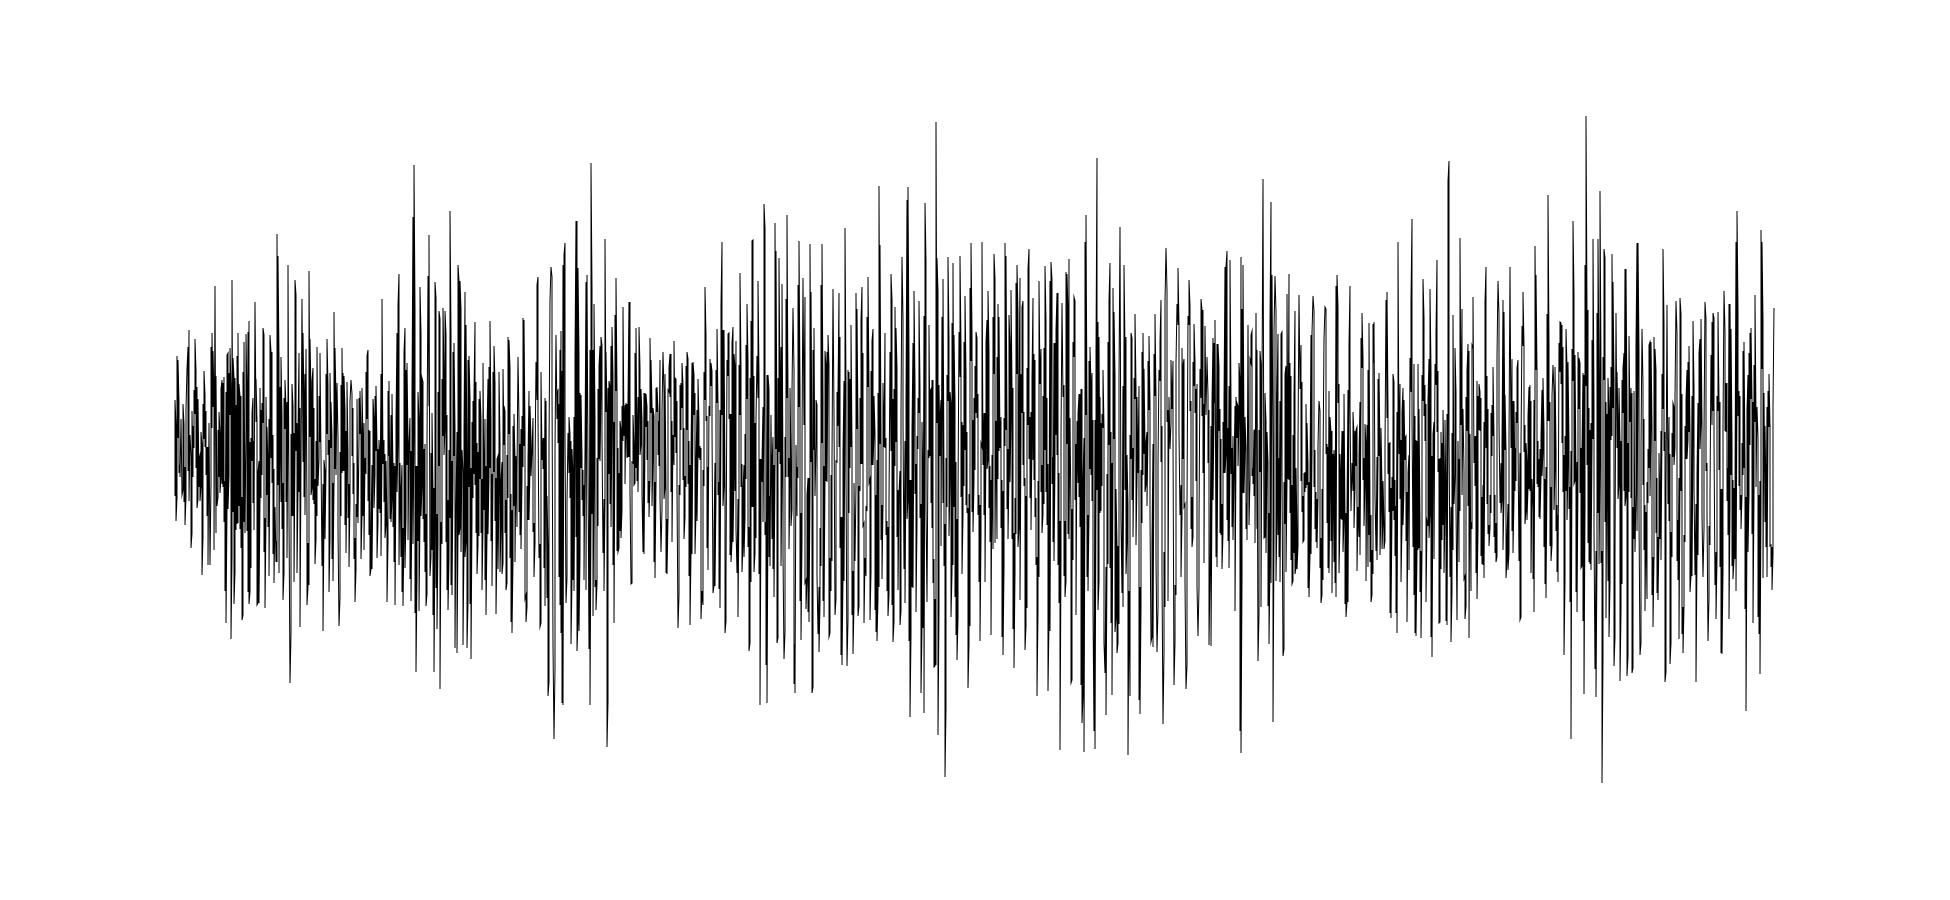
\includegraphics[width=0.45\textwidth]{figure/single-channel-animals.png}
  \caption{A waveform composed of multiple sound sources (cf. Fig. \ref{fig:animal_multichannel}).}
  \label{fig:animal_singlechannel}
\end{wrapfigure}
%
It is composed of all environmental sounds contributing to the air pressure fluctuation at the tympanic membrane\footnote{Note that this is for illustration purposes; the waveform will obviously look different when shaped by a given environment and the human ear canal before reaching the tympanic membrane.}.

However, using the framework of auditory scene analysis, the human auditory system is able to separate this input signal into its various sources, or ``auditory objects''.  In effect, this would separate the above waveform into its actual component sources of human speech, and the sounds of a sheep, cow, and horse, seen in Figure \ref{fig:animal_multichannel}; ``The normal auditory system exhibits a remarkable ability to parse these complex scenes'' (\cite{middlebrooks:17}, 2).

Of course, there reaches a point at which the auditory system fails and can
%
\begin{figure}[h]
\centering
  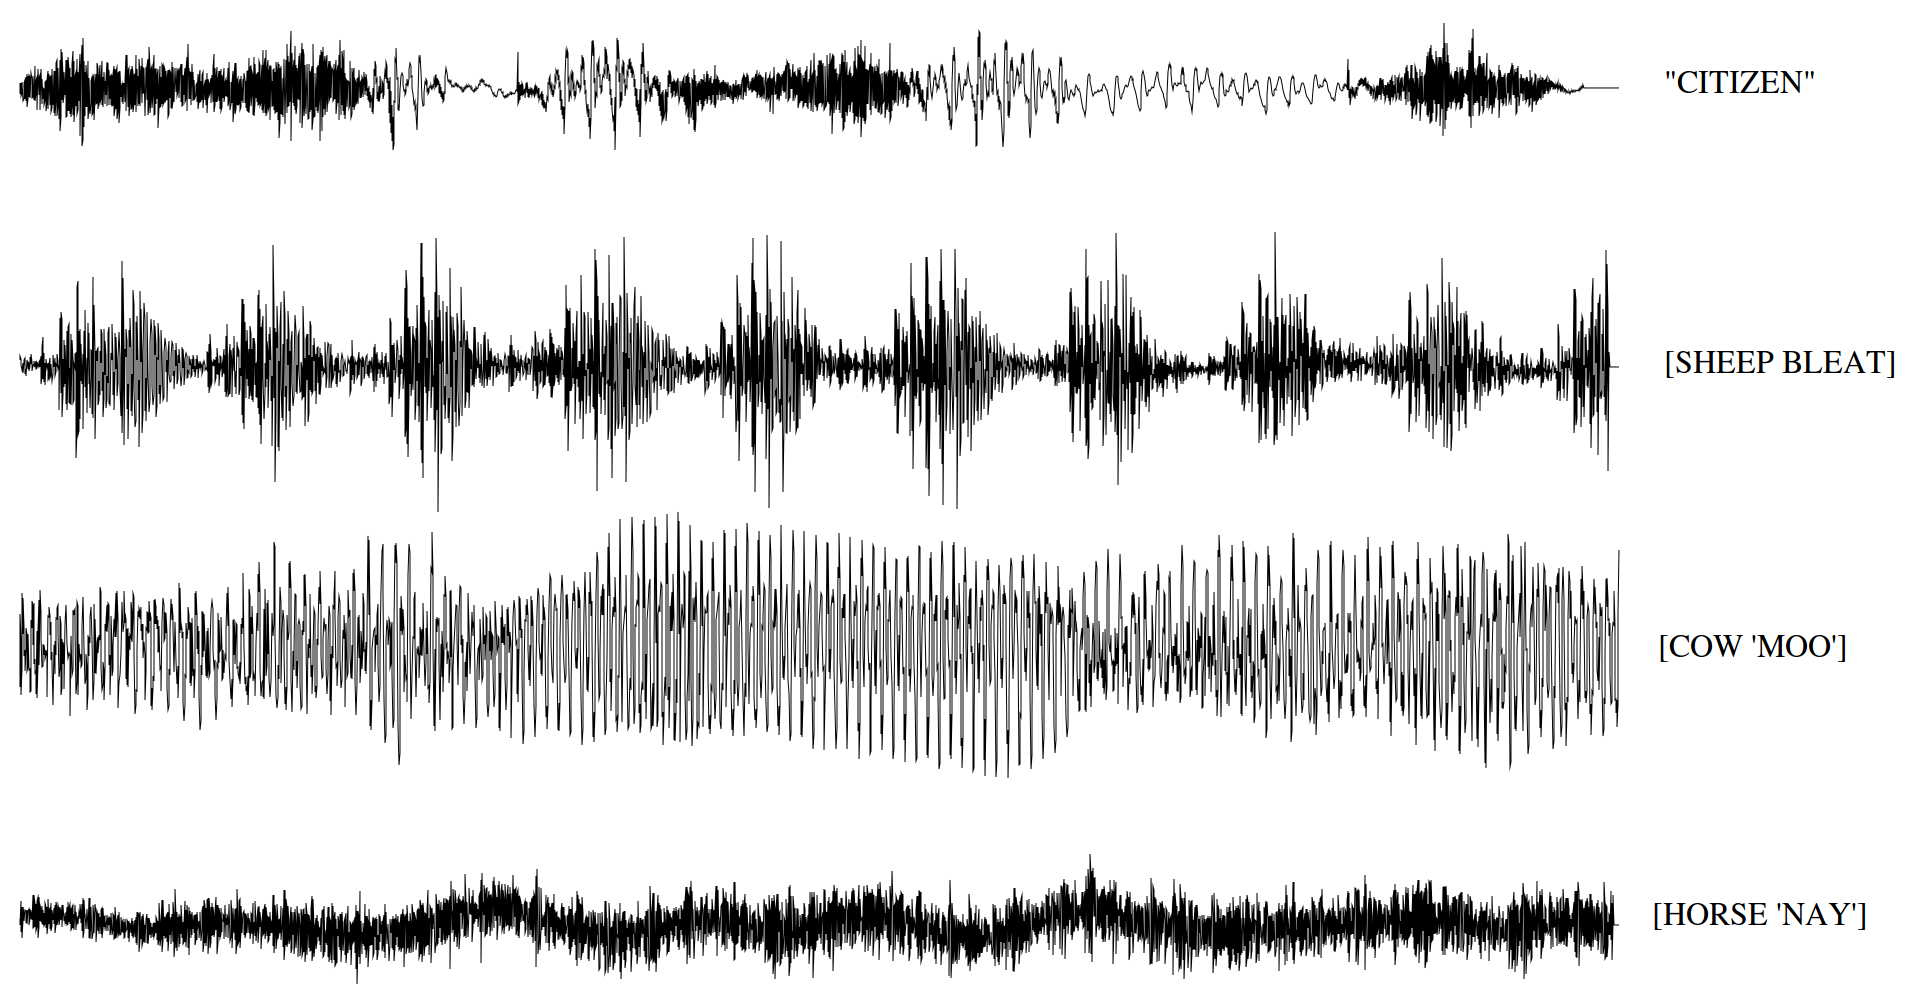
\includegraphics[width=0.95\textwidth]{figure/multi-channel-animals_w-text.png}
  \caption{The four component waveforms (human speech, sheep, cow, horse), of the combined waveform seen in Figure \ref{fig:animal_singlechannel}.}
  \label{fig:animal_multichannel}
\end{figure}
%
 no longer differentiate all sources, or, more relevant to this paper, recognize the information in a human speech signal when embedded with background noise from one or more additional sources.  The following section will describe in more depth the acoustics of speech in noise.
  
\subsection{Acoustics of Speech in Noise}
\label{bkgrnd:speech_in_noise}

Speech in noise can be intuitively grouped into two components, the speech (more specifically the voice one is intending to hear) and the noise, called the ``masking'' element.  Broadly, masking can be defined as ``the process by which the threshold of hearing for one sound is raised by the presence of another'' (\cite{ansi:13}, 61).  This masking element is anything \textit{but} the voice\footnote{For the purposes of this paper, the term ``voice'' will be used throughout to refer to the singular speech source the listener desires to hear out of the masked signal.} (speech signal) that one is interested in, as it was intended to be heard.
%which, as indicated in Chapter 2\ref{chapter2}, could be of any form or loudness.

The masking process can be broken down into two forms: energetic masking and informational masking.  Energetic masking occurs when the masking element shares the same temporal and frequency elements of the voice.  It can be thought of as if the masked element and the voice are competing for ``space'' along the basilar membrane and then the auditory nerve (\cite{brungart:01}), but can also be considered to be competing for the listener's attention (ie. the listener must concentrate on ignoring the mask, and exclusively listening to the target, (\cite{mattys:12})).  Energetic masking is normally thought to occur primarily in the ``lower'' auditory processes, eg. the cochlea and auditory nerve, though this is not always the case, as described further below.  

Informational masking can be broadly thought of as difficulties relating to memory, linguistic processing, and the like, oftentimes generalized to speech-on-speech noise.  \cite{mattys:10} failed to find informational masking in a cross-linguistic task, and so it is possible that informational masking could be limited to situations in which the masking speech is intelligible. This type of masking is thought to occur primarily in the ``higher auditory processes'' in the brain.

An instance of both energetic and informational masking can be visualized in a diagram of overlapping speech presented in \cite{middlebrooks:17}, and seen in Figure \ref{fig:sos-masked-spctgrms}.
%
\begin{figure}
\centering
  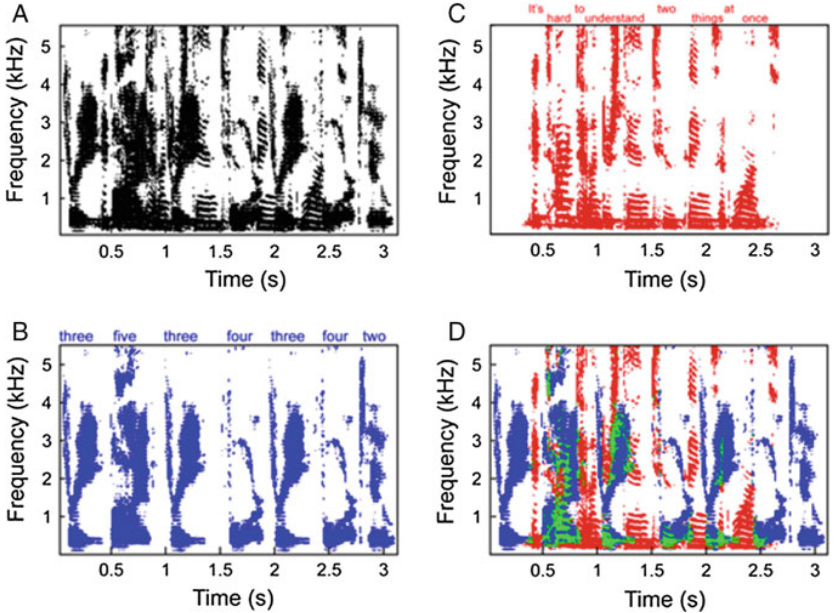
\includegraphics[width=0.95\textwidth]{figure/speech-on-speech_masked_spectrograms.png}
  \caption{Diagrams of different spectograms. (A) The spectogram of two temporally overlapping spoken utterances. (B) The spectogram of the utterance ``three five three four three four two'' colored in blue (C) The spectogram of the sentence ``It's hard to understand two things at once.'' colored in red. (D) The overlap of the two spectograms (B) and (C), with the color green highlighting the areas of energy in frequency and time that overlap. }
  \label{fig:sos-masked-spctgrms}
\end{figure}
%
Say that utterance (C) in the figure is the desired ``voice'', leaving utterance (B) the masking element.  In (D), one can see the voice (red), the areas of masking in which there is direct frequency and temporal overlap (green), and the remainder of the masking speech (blue). Of course this is never so nicely differentiated, and the resulting acoustic information that the auditory system gets can be seen in (A), in which no source is differentiated.  This could primarily be viewed as a form of energetic masking (competition for lower-level processing), though upper level processing is required to take meaning from the desired voice, which is masked informationally by the other, competing voice carrying its own information.

The five different background noises used in the study described in Chapter 2\ref{chapter2} primarily serve the purpose of energetic masking of the voice in the signal.  A small (5 second) portion of the spectrogram of each sound can be seen in Figure \ref{fig:bkgrnd-noises}.  These sounds don't produce any competing linguistic informational content themselves which mask the desired voice (the `cafe' noise, seen in Figure \ref{fig:cafe-bkgrnd}, does contain speech babble, none of it intelligible), and so masking occurs by producing energy at the same time as - and in the same frequency range as - the recorded voice.

\begin{figure}[h!]
\begin{subfigure}{0.475\linewidth}
  \centering
  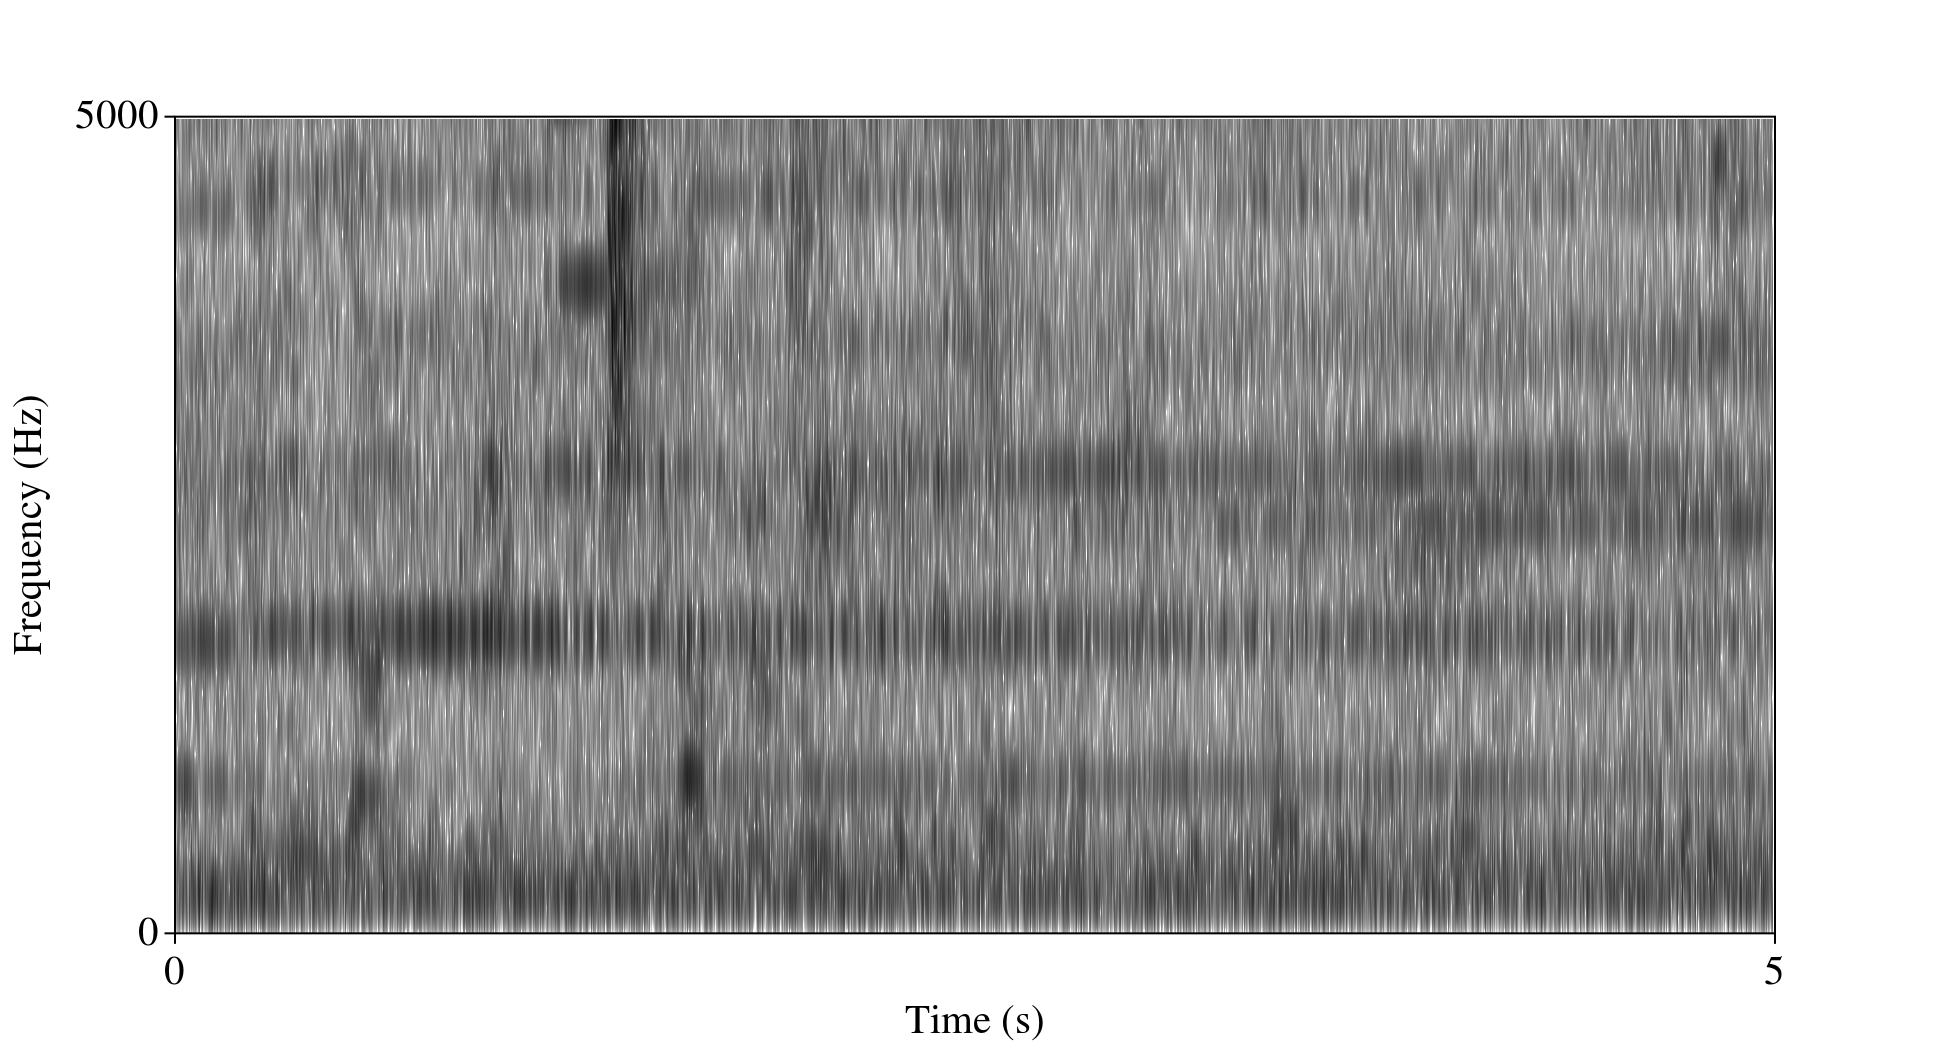
\includegraphics[width=0.9\textwidth]{figure/spctgrm-bus-background.png}
  \caption{Bus background noise.}
  \label{fig:bus-bkgrnd}
\end{subfigure}
\qquad
\begin{subfigure}{0.475\linewidth}
  \centering
  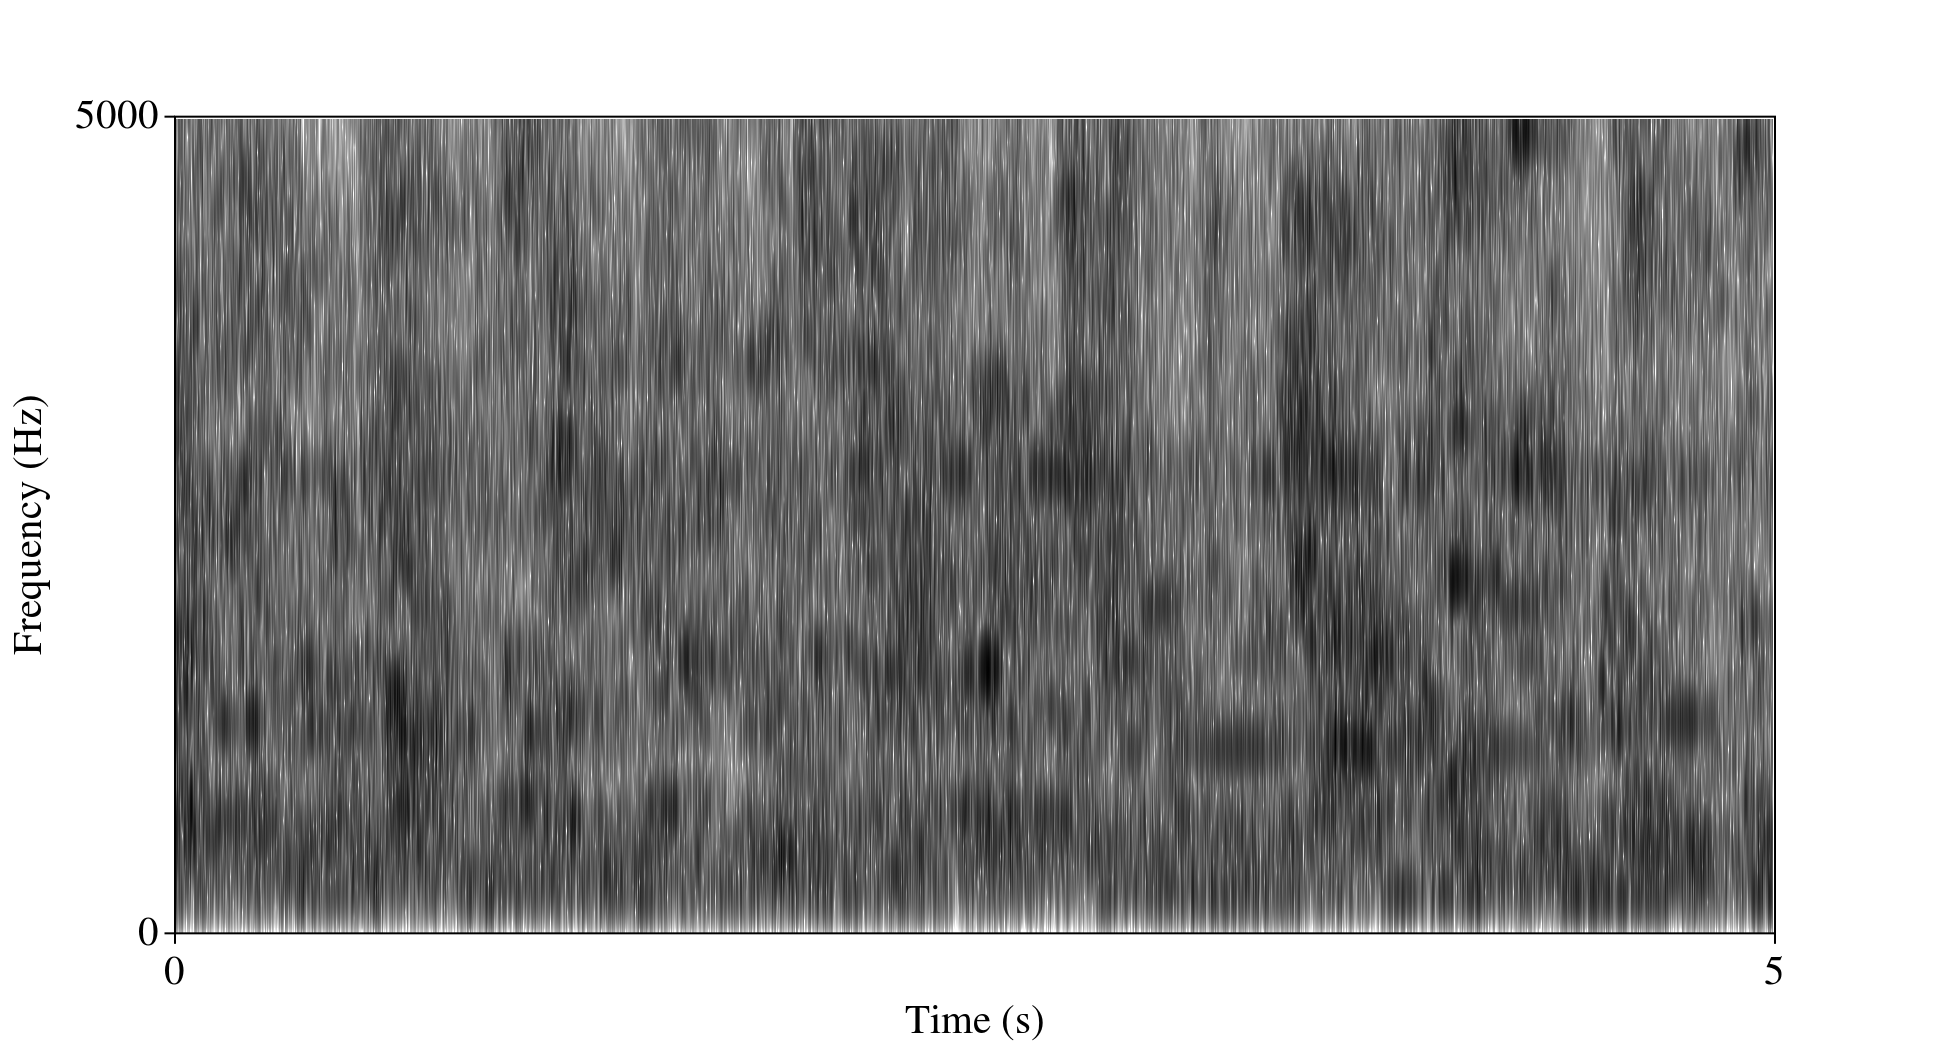
\includegraphics[width=0.9\textwidth]{figure/spctgrm-cafe-background.png}
  \caption{Cafe background noise.}
  \label{fig:cafe-bkgrnd}
\end{subfigure}%
%\hfill
\\[2ex]
\begin{subfigure}{0.475\linewidth}
  \centering
  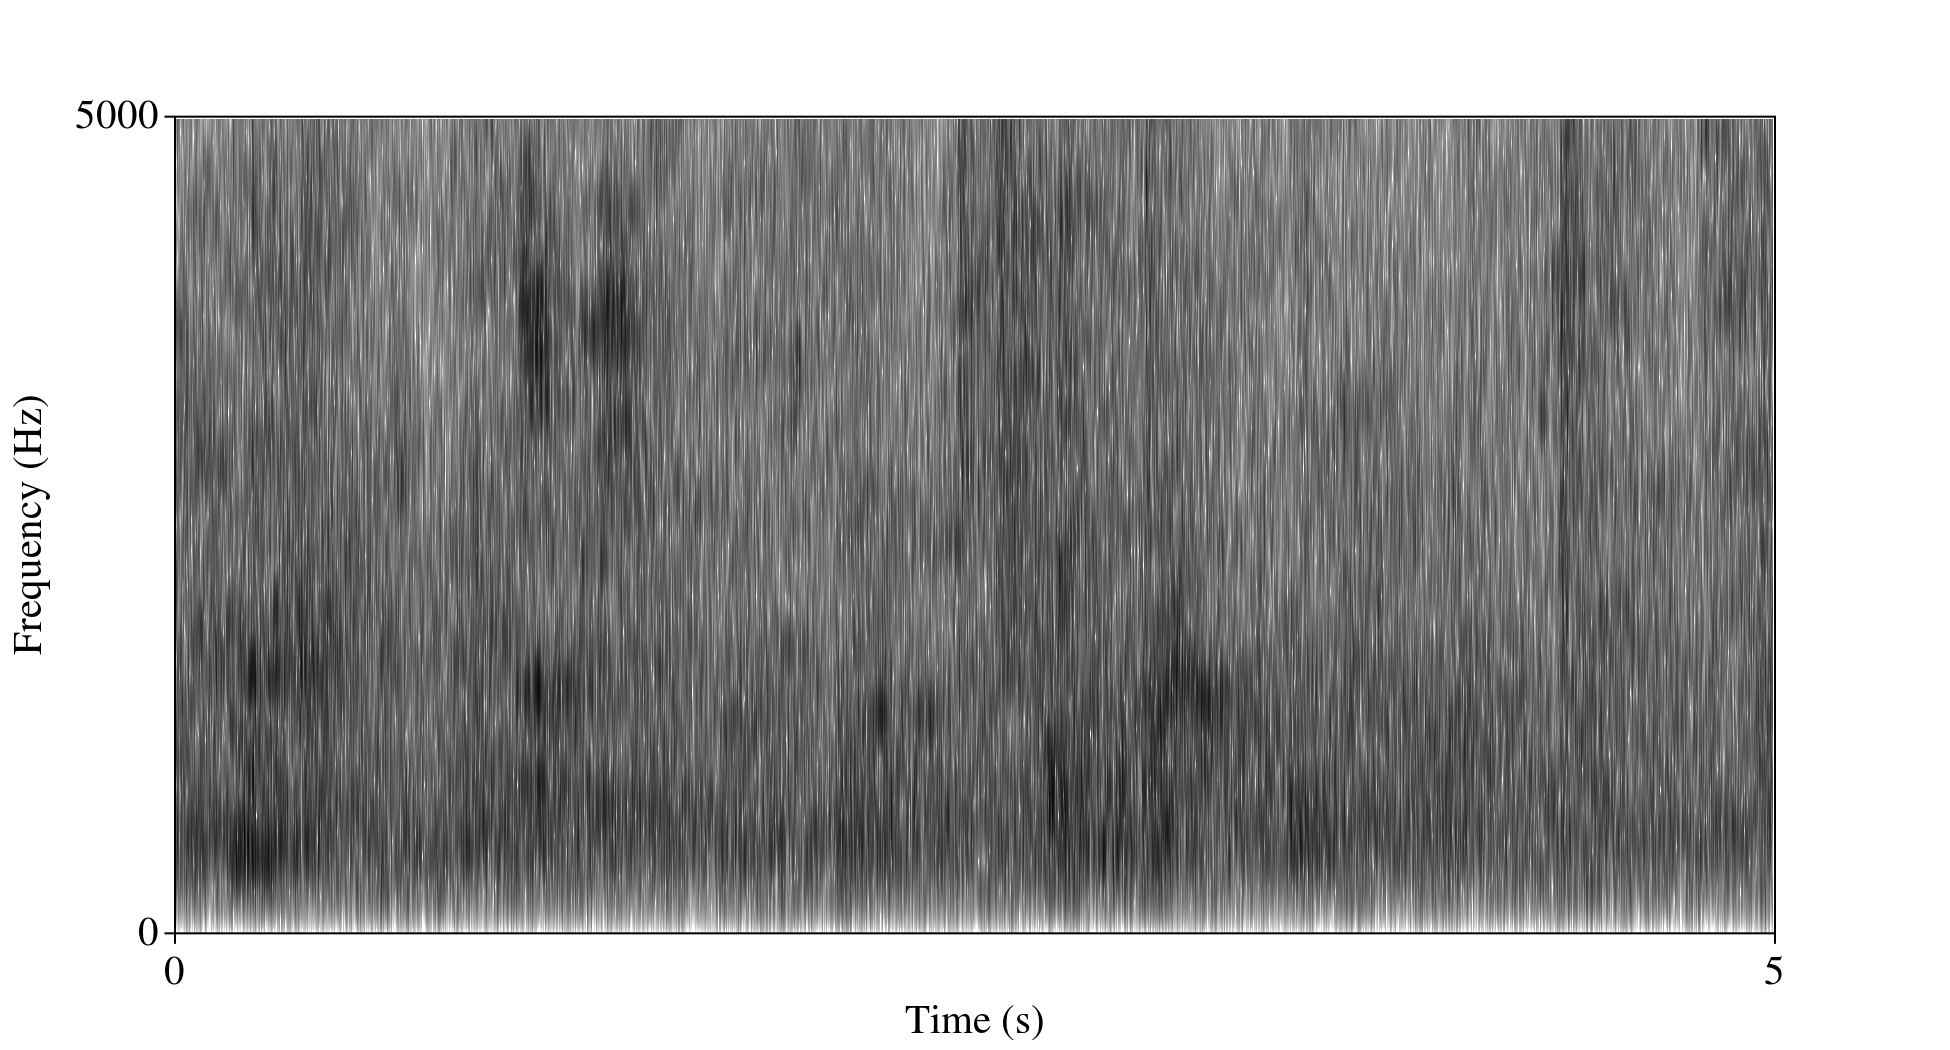
\includegraphics[width=0.9\textwidth]{figure/spctgrm-ped-background.png}
  \caption{Pedestrian background noise.}
  \label{fig:ped-bkgrnd}
\end{subfigure}
\qquad
\begin{subfigure}{0.475\linewidth}
  \centering
  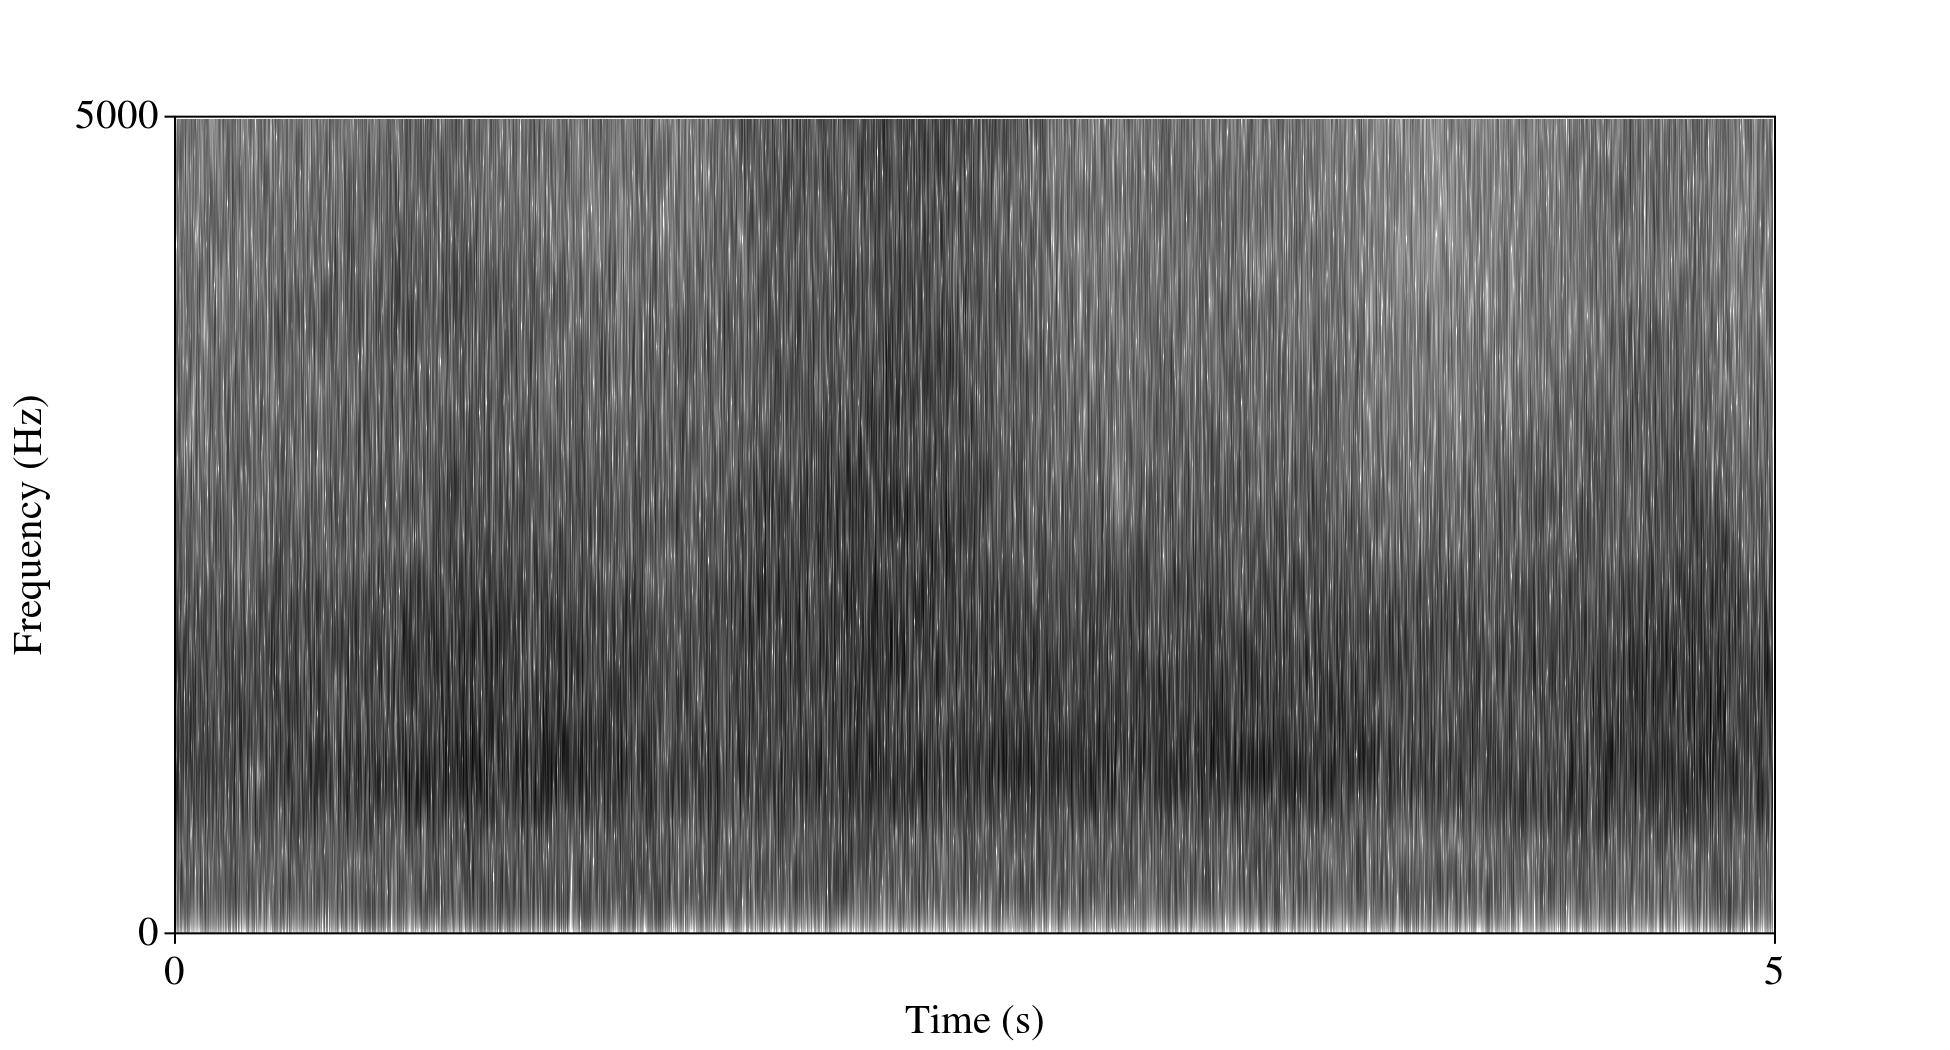
\includegraphics[width=0.9\textwidth]{figure/spctgrm-str-background.png}
  \caption{Street background noise.}
  \label{fig:str-bkgrnd}
\end{subfigure}%
%\hfill
\\[2ex]
\begin{center}
\begin{subfigure}{0.475\linewidth}
  \centering
  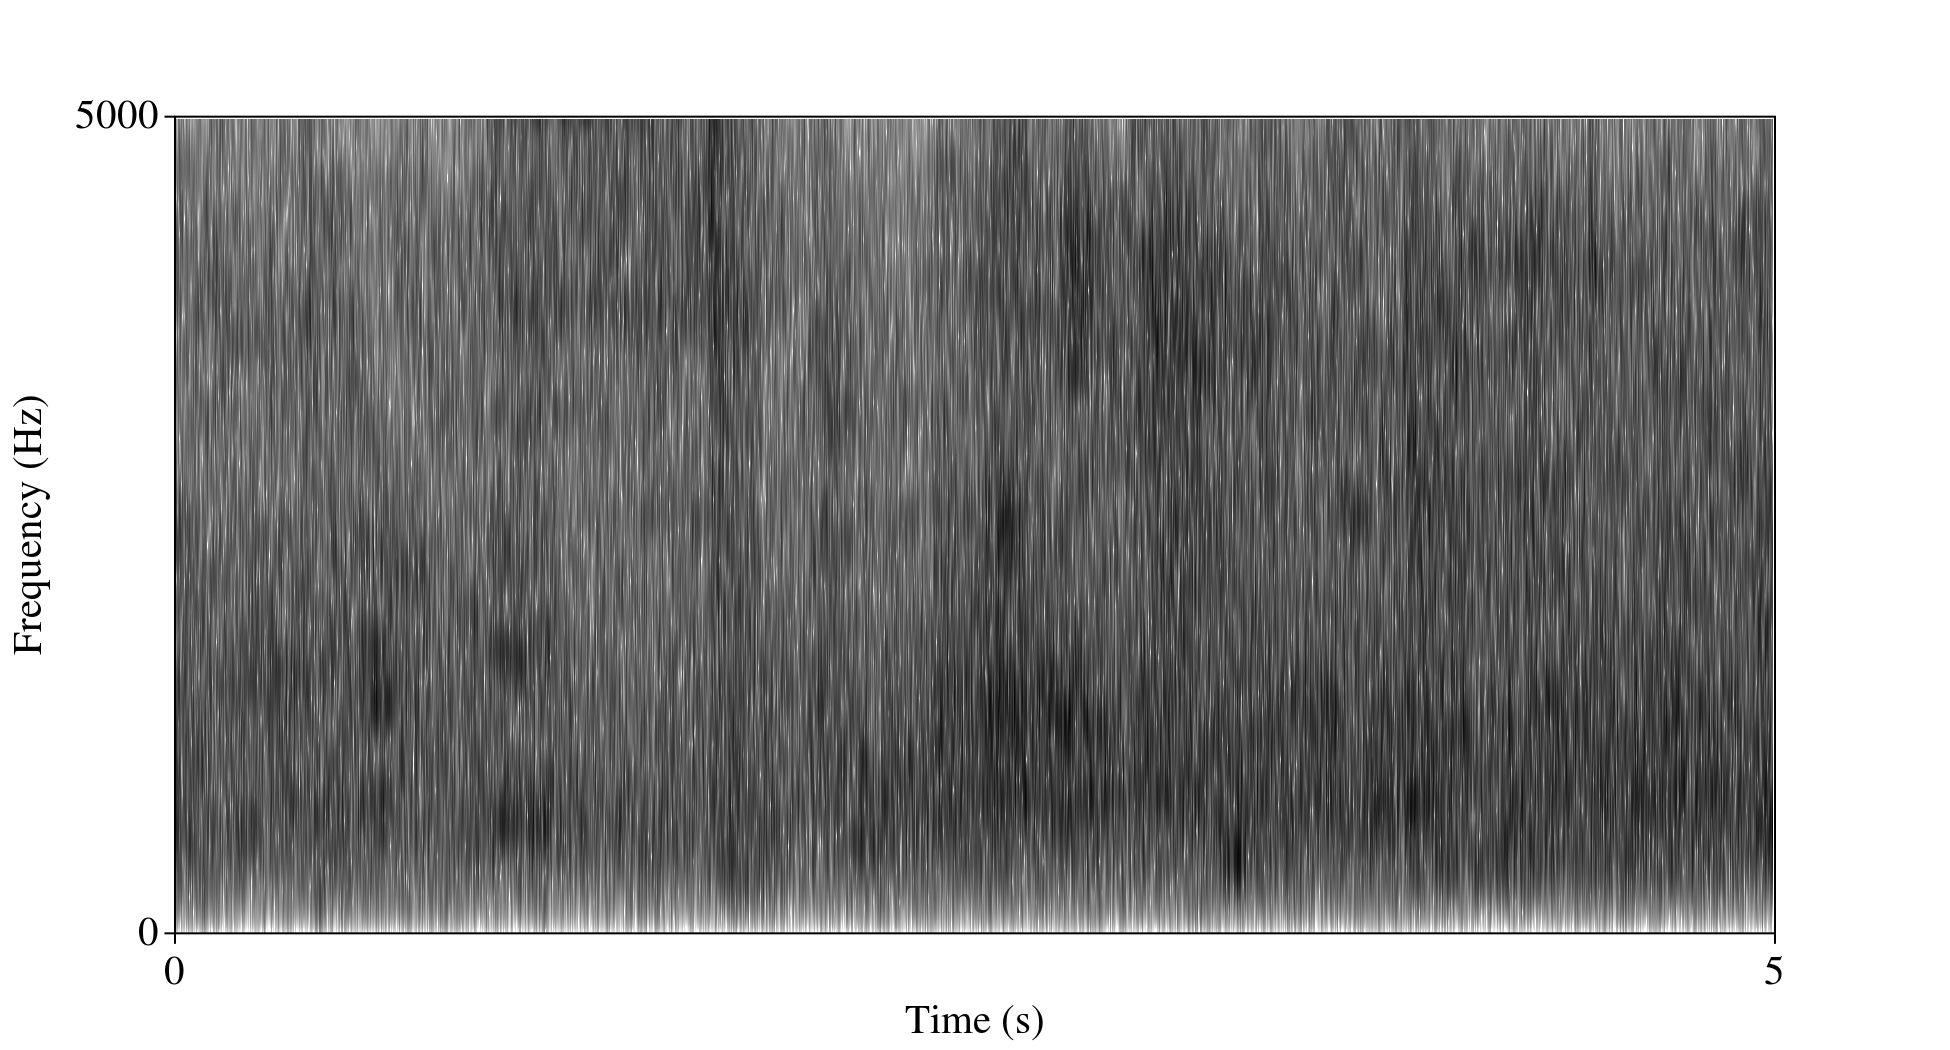
\includegraphics[width=0.9\textwidth]{figure/spctgrm-fac-background.png}
  \caption{Factory background noise.}
  \label{fig:fac-bkgrnd}
\end{subfigure}
\end{center}
\caption{Example spectograms of the first five seconds of the background noise tracks. Most recorded sentences occurred within these temporal spans.}
\label{fig:bkgrnd-noises}
\end{figure}

Yet simply because a sound may be ``masked'' does not necessarily imply that the voice is not heard or understood.  There are a number of methods used by the auditory system to overcome the masking and interpret the voice; this process is termed ``release from masking'' (\cite{middlebrooks:17}).  One such proposed method, the use of humans' built in binaural hearing, uses both ears to tease apart the different sources, utilizing the very small temporal difference that occurs when different sound sources reach each ear.  
In this example, it is easy to see that energetic and informational masking are not strictly limited to masking separate ``lower'' and ``higher'' processes (\cite{durlach:06}).
The use of binaural hearing is an example of utilizing a ``higher'' process as a release from energetic masking, as it necessarily requires signals from both ears to be interpreted (\cite{hirsh:48}). Binaural hearing is essentially making use of the spatial directionality of the noise(s) from the listener to separate the different sources (\cite{bregman:94}).

There are many other proposed methods of release from energetic masking. One involves making note of acoustic transitions: ``when [a] sound...changes its properties gradually, [it] is likely to be heard as a single changing sound.  However, when [it] changes...abruptly, [it] tends to be treated as a newly arriving sound, this tendency increasing with the abruptness of the change.'' (\cite{bregman:94}, 5).  The use of fundamental frequency (F0) has also been shown to be an effective tool, presumably to interpret the location of harmonics, and parse apart different sources (eg. two separate, simultaneous vowels with different F0s, (\cite{bird:97})). There are many other proposed methods to release masking that the auditory system uses, particularly among informational masking (\cite{middlebrooks:17}), but these are beyond the scope of this project.


\subsection{Performance of Human Recognition of Speech in Noise}

Eventually, however, with enough background noise and masking, the methods listed above for releasing the masking will fail and recognition will begin to break down.  Under the most simple conditions to measure - steady-state noise - \cite{ding:13} report that when listening to speech in noise, human self reported intelligibility ratings don't drop significantly until the SNR reaches approximately -3 dB, where intelligibility drops to about 55\%, and it doesn't hit near floor level (0\%) until -9 dB SNR.

This subjective measure is backed by a study performed by \cite{gilbert:13}, who used the PRESTO corpus (\cite{garofolo:93}) to test sentence intelligibility among 121 native English speakers.  \cite{gilbert:13} found that - similar to \cite{ding:13} - the median score (at the 50th percentile) of speech with a -3dB SNR had about 55\% accuracy.  At +3 dB SNR, the median score increased to approximately 88\% accuracy.

\cite{ding:13} do however mention that there was great inter-speaker variation among the reported subjective perception of intelligibility of an utterance; this is also supported by \cite{gilbert:13}'s results. They showed that, averaging over all SNR conditions (-5, -3, 0, +3 dB), the variability between speaker's accuracy scores had a range of almost 36\% for a given item.  A retest performed with a subgroup of the original participants on the same dataset yielded a similar (~34\%) range of variability in accuracy.  

\cite{francis:10} discusses how listening to speech in background noise places extra demands on working memory, as does listening to degraded speech (\cite{francis:09}).  The diversion of working memory to acoustic processing can be particularly detrimental to performance when simultaneously working on other computation, e.g. syntactic and semantic parsing (\cite{caplan:99}), such as in phrase or sentence recognition. \cite{tamati:13} tested a group of high-performing hearers of speech in noise against a separate group of low-performing hearers using several different working- and short-term memory tasks.  Not surprisingly, the group of listeners who are able to better hear speech in noise also perform statistically better on the working memory tasks.  Working- and short-term memory are by no means the only indicators of perceptual performance.

\cite{mattys:12} briefly discusses the concept of perceptual learning, which asserts that one can learn to accommodate a particular adverse condition (eg. background noise, signal distortion, etc.) with practice in that area.  Learning will be less effective in cases which the degradation is variable or unpredictable between trials, such as with unpredictable background noise.  The speech with the background noises in this present study will be presented in a random order, and since the background noise varies, it cannot be assumed or predicted from one sentence to the next, and therefore likely will not be `learned' in this sense.

Although there is expected to be a great amount of variability between subjects, the results from the \cite{ding:13} and \cite{gilbert:13} studies indicate that the average SNR for the highest noise condition from the data collected and described in Chapter 2\ref{chapter2}\footnote{Some of the lowest 80 dB noise condition sentences yielded approximately +6dB SNR} is over 9 dB SNR above the 50\% intelligibility threshold at -3 db SNR given by these two studies.  It is unlikely that listeners will encounter much masking in the collected noisy speech that won't be overcome.

After testing two pilot participants on the speech collected, it was deemed that the speech in the noisy background (described in Chapter 2\ref{chapter2}) was too easily recognizable.  This conclusion was drawn because the average performance on noisy speech (using word error rate\footnote{The lower the error rate, the more accurate}) was at a very low 10\% using only the 80 dB noise condition; the average non-noisy mouth-recorded speech was only slightly more accurate at 7\% word error rate. The cause was likely that the SNR ratio was not low enough, as explained in Section \ref{ch2:limitations}.  Due to this, two additional participants were rerun with lower SNRs, explained more in Section \ref{expt2}.

%Experiment redo

% Rediscuss these (learning directly above, cover briefly) in brief background when introducing secondary studies)
%PERCEPTUAL LEARNING AS IMPETUS FOR READING TRAINING TASK
%FREQUENCY as release of energetic masking AS IMPETUS FOR COMBINATION STIMULI


\section{Experiment 3: Human Speech Perception in Noise}
\label{expt3}

After additional stimuli were gathered from two additional participants (explained below in Section \ref{chap4:methods:stimuli}), a human speech perception experiment was run on the data in order to better understand and compare the ability of the auditory system to accurately comprehend the speech with a noisy background and the [modified] speech distorted by passage through the speaker's head.  To act as a control, participants would also listen to the normal, clean speech.

\subsection{Stimuli Generation}
\label{chap4:methods:stimuli}

To remedy the problem of the noisy speech being \textit{too} intelligible and having a high SNR, 
%
\begin{wrapfigure}{r}{0.5\textwidth}
\centering
  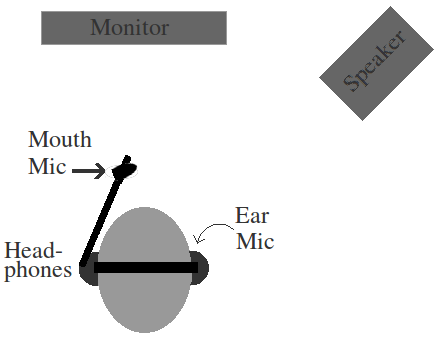
\includegraphics[width=0.45\textwidth]{figure/overallSetUp_new.png}
  \caption{This is the same setup as described in Chapter 2\ref{chapter2}, except that the mouth microphone is facing the loudspeaker, rather than the mouth.}
  \label{fig:overallSetUp_new}
\end{wrapfigure}
%
two additional participants (one male, one female) were recorded following the procedure in the first task (cf. Chapter 2\ref{chapter2}).  The list of stimuli was increased to 80 sentences (eight Harvard Sentence lists\footnote{This included the previous three lists, 14, 28, and 57, as well as lists 21, 29, 37, 53, and 68. These additional lists were pseudo-randomly chosen, as were the original three lists, to contain words that would be readily recognizable by the participant population.}) to provide more reaction data from this present experiment.  

To increase the SNR, the directional microphone was pointed away from the mouth of the participant, and directed toward the loudspeaker (see Fig. \ref{fig:overallSetUp_new}).  This, of course, results in some of the limitations outlined in Section \textit{\textbf{[Chapter 2: Limitations]}}\ref{ch2:limitations} in Chapter 2\ref{chap2}; for example, simply pointing the mouth microphone toward the loudspeaker, rather than increasing the noise, ignores the fact that the noise level inside the ear canal might increase as well with an increase in ambient noise.  Given the alternatives outlined in Section \ref{ch2:limitations}, this was seen as the best available option.  Figures \ref{fig:spectNewMouthNoise} and \ref{fig:spectNewEarNoise} show the new noisy and ear recorded speech, respectively.
%
\begin{figure}
\begin{subfigure}{0.5\textwidth}
  \centering
  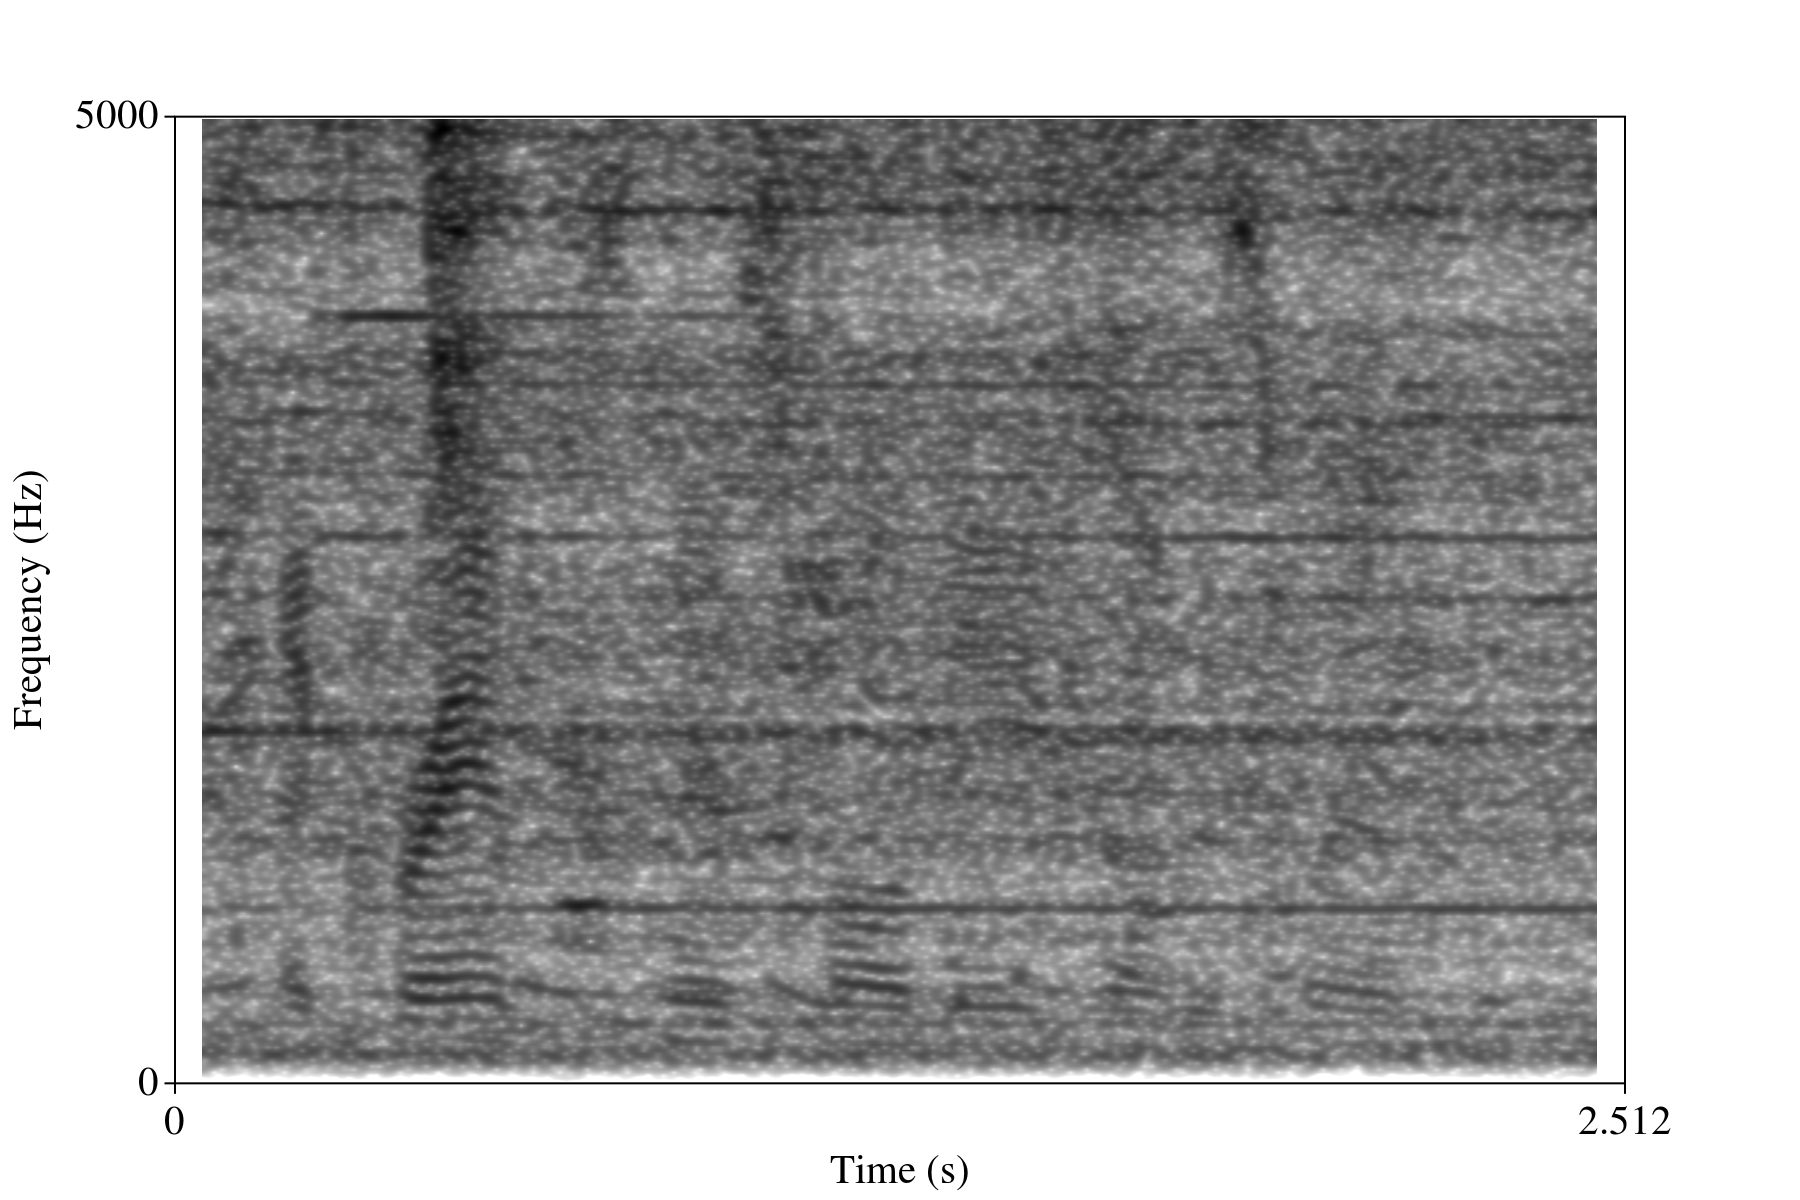
\includegraphics[width=0.9\textwidth]{figure/spectNewMouthNoise.png}
  \caption{New recording at the mouth with the microphone pointed toward the loudspeaker noise source.}
  \label{fig:spectNewMouthNoise}
\end{subfigure}
%
\begin{subfigure}{0.5\textwidth}
  \centering
  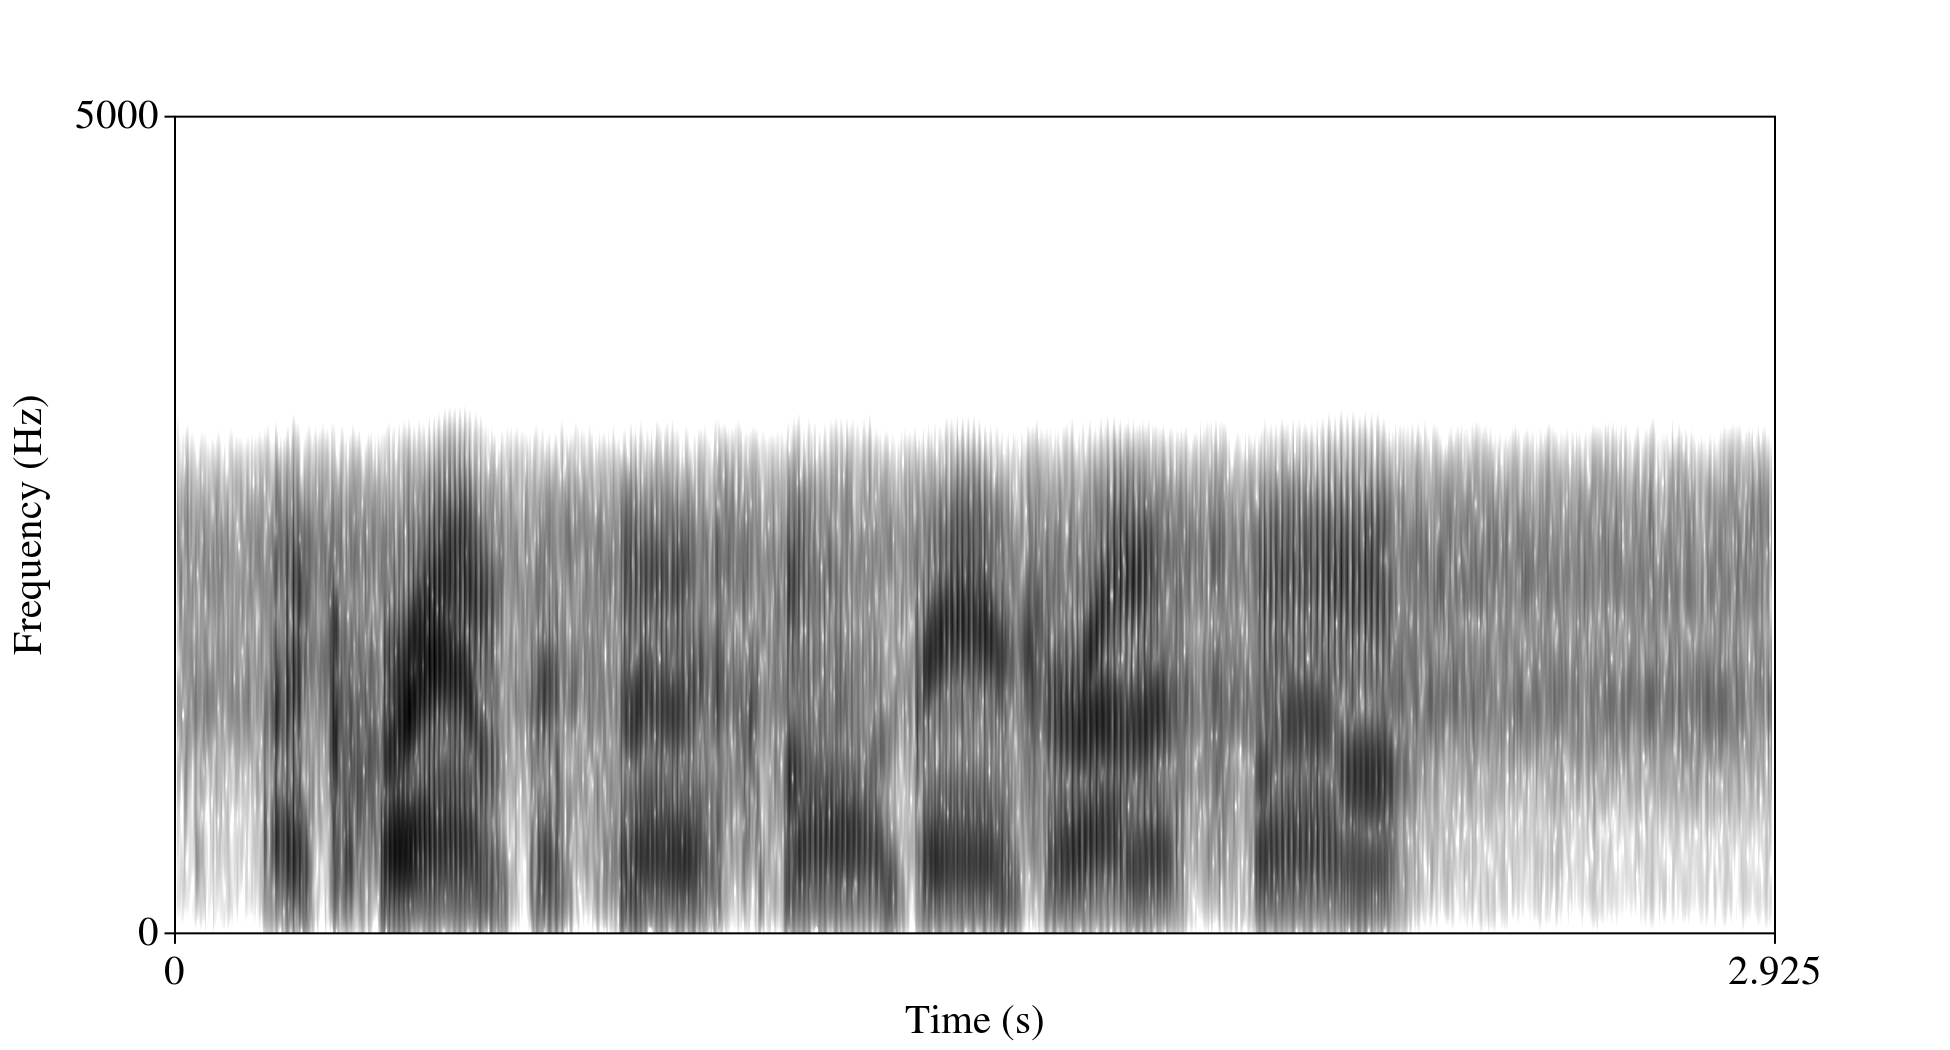
\includegraphics[width=0.9\textwidth]{figure/spectNewEarNoise.png}
  \caption{New recording at the ear; all recording conditions for the ear were the same as in the first group of recordings.}
  \label{fig:spectNewEarNoise}
\end{subfigure}
\caption{The sentence ``A cramp is no small danger on a swim'' spoken by the male speaker, recorded at the mouth (Fig. \ref{fig:spectNewMouthNoise}) with ``cafe'' noise, and simultaneously at the ear (Fig. \ref{fig:spectNewEarNoise}).}
\end{figure}


Furthermore, due to the issue of the lack of noise in the noisy speech signals, only one noise level condition was used - the highest available noise level (80 dB).  All previously used background noise types were used for this data collection task as well.


\subsection{Design}
\label{chap4:methods:design}

The experiment had three factors - gender of speaker\footnote{This has been included to ensure there is no effect of gender on perception in noise or on transmission of speech through the head and into the ear canal, due to the difference in male and female vocal tracts.} \textbf{x} microphone location \textbf{x} noise type - resulting in a 2x2x6 experiment.  There were two genders, two mic locations (recording at the ear, and at the mouth), and six noise types (bus, cafe, pedestrian, street, factory, and no noise (clean)).  Since the ability to understand speech in noise is quite variable between individuals, the design of this experiment was a within-subjects experiment.  This meant that each of the 2x2x6 (ie. 24) conditions needed to be seen by each participant.  The sessions that were re-recorded utilized 80 distinct sentences, which allowed for three sentences to appear in each of the 24 conditions, totaling 72 sentences used in the experiment.  The eight remaining sentences were used as a ``training'' set, intended to get the participants used to the task itself, rather than to acclimate them to the type of speech that they would hear.

Since any given speaker could not hear the same sentence twice without introducing a confound, and since each sentence was recorded in each of the 24 conditions\footnote{72 distinct sentences * 24 conditions = 1728 total sentence recordings}, this necessitated the use of 24 co-balanced groups to ensure that each sentence was heard in every condition by at least one speaker.  For example, sentences 1, 2, and 3 would occur in Factor Combination \#1 (e.g. female speaker, mic at the mouth, with bus background noise) in co-balanced group \#1 for Participant \#1. Participant \#2 would see co-balanced group \#2, which placed sentences 1, 2, and 3 in Factor Combination \#2 (e.g. female speaker, mic at the mouth, with cafe background noise).  For simplicity's sake, each grouping of three sentences would appear together in a given condition, and were not mixed up between the different co-balanced groups.  However, once the sentences are assigned to a particular condition, the order of presentation to the participants is randomized.

\subsection{Participants}

Twenty-four native speakers of English with self-reported normal hearing participated in the experiment. Each participant was placed into a separate co-balanced group, as specified above in Section \ref{chap4:methods:design}.

\subsection{Equipment}

The experiment was conducted in a soundbooth with a pair of over-the-ear headphones.  The experiment interface utilized in-house developed software, and participants' answers were typed into a textbox in this program, on a computer whose monitor could be seen from inside the soundbooth.

\subsection{Procedure}
\label{hsp-main-procedure}

The participant was seated in the sound booth in front of a keyboard and computer monitor with a pair of headphones, and was given a set of instructions. They were told that they would hear each utterance only once, and what they would hear was comprised of real English words, but may not constitute a ``complete'' sentence.  They were forewarned that many of the sentences they would hear would be noisy and difficult to understand. They were instructed to write all words they heard, even if what was heard did not make syntactic sense, or if the words were not adjacent (e.g. if only the first and last word of the sentence was heard). They would be timed, with 18 seconds to type their response starting from the beginning of the sound file and that their answer would be saved as-is if they ran into the time limit, preventing them from typing more.

The participant was told that the first set of eight utterances they heard were part of a ``training'' set of eight utterances intended to familiarize them with the task\footnote{The same eight sentences were heard by every participant}.  None of the utterances from the training set were used in the analysis.  Once completed with this initial set, participants were asked if they had any questions.  Afterwards they began the primary task in the soundbooth.  They would hear one of the sentences, and type their answer in a text box.  When finished with their answer, they would either click to advance to the next sentence, or, if they ran into the time limit, were prevented from modifying their answer, and were prompted to click another button to advance.  When finished with all 72 stimuli, the participant was given a brief questionnaire to fill out.  

After the experiment, the researcher would double check participant answers for correct spelling.  Only obvious errors were modified (e.g. `teh' to `the', `crakers' to `crackers', `mantle' to `mantel'), while ambiguous errors were left as-is (e.g. `blo' was not changed to `block', `finde' was not changed to `fine').  Numbers were also lexicalized (e.g. `30' to `thirty').  Punctuation was removed for ease of analysis and calculation of word error rate.  Exact responses given by each participant can be found in Appendix F\ref{appendixF}.


\section{Results}
\label{ch4:results}



The word error rate (WER) for each (spell-checked) response for each participant was calculated. The code for the WER calculation can be found in Appendix F\ref{appendix?}

A 3-way, within-subjects ANOVA was performed with the collected data - 72 sentences from each of the 24 participants. Factors included the gender of the speaker (of the stimulus) with two levels - male and female - the location of the recording microphone with two levels - at the mouth and at the ear - and the background noise type with six levels - no noise, bus noise, cafe noise, pedestrian noise, street noise, and factory noise.  There was no significant 3-way interaction between speaker gender, noise type, and mic location, as can be seen in the by-subjects ANOVA (Table \ref{tab:anova1_by_subj}) and the by-items ANOVA (Table \ref{tab:anova1_by_item}). Two, two-way interactions were significant, speaker gender \textbf{x} mic location, and noise-type \textbf{x} mic location. The two way interaction between speaker gender and noise type was not significant.  The main effects of all three factors were also significant (cf. Tables \ref{tab:anova1_by_subj} and \ref{tab:anova1_by_item}).

% latex table generated in R 3.4.1 by xtable 1.8-2 package
% Sun Jul  9 18:16:31 2017
\begin{table}[ht]
\centering
\begin{tabular}{lrrrrl}
  \hline
Effect & DFn & DFd & F & p & p$<$.05 \\ 
  \hline
speaker\_gender & 1.00 & 23.00 & 6.69 & 0.02 & * \\ 
  noise\_type & 5.00 & 115.00 & 84.83 & 0.00 & * \\ 
  mic\_location & 1.00 & 23.00 & 155.07 & 0.00 & * \\ 
  speaker\_gender:noise\_type & 5.00 & 115.00 & 0.55 & 0.74 &  \\ 
  speaker\_gender:mic\_location & 1.00 & 23.00 & 18.53 & 0.00 & * \\ 
  noise\_type:mic\_location & 5.00 & 115.00 & 55.53 & 0.00 & * \\ 
  speaker\_gender:noise\_type:mic\_location & 5.00 & 115.00 & 1.61 & 0.16 &  \\ 
   \hline
\end{tabular}
\caption{ANOVA for by-subjects analysis of the three-factor, within-subjects experiment.} 
\label{tab:anova1_by_subj}
\end{table}
% latex table generated in R 3.4.1 by xtable 1.8-2 package
% Sun Jul  9 18:16:32 2017
\begin{table}[ht]
\centering
\begin{tabular}{lrrrrl}
  \hline
Effect & DFn & DFd & F & p & p$<$.05 \\ 
  \hline
speaker\_gender & 1.00 & 71.00 & 4.01 & 0.05 & * \\ 
  noise\_type & 5.00 & 355.00 & 103.50 & 0.00 & * \\ 
  mic\_location & 1.00 & 71.00 & 354.53 & 0.00 & * \\ 
  speaker\_gender:noise\_type & 5.00 & 355.00 & 0.52 & 0.76 &  \\ 
  speaker\_gender:mic\_location & 1.00 & 71.00 & 21.36 & 0.00 & * \\ 
  noise\_type:mic\_location & 5.00 & 355.00 & 71.03 & 0.00 & * \\ 
  speaker\_gender:noise\_type:mic\_location & 5.00 & 355.00 & 1.86 & 0.10 &  \\ 
   \hline
\end{tabular}
\caption{ANOVA for by-items analysis of the three-factor, within-subjects experiment.} 
\label{tab:anova1_by_item}
\end{table}



Mauchley's Test for Sphericity\footnote{Sphericity assumes that the variance between levels of a factor are the same; sphericity is violated when this is not the case.} was conducted, both for the by-subjects and by-items ANOVAs.  Significant sphericity violations were found for the main effect of noise type, and the interaction of speaker gender and noise type, as can be seen in Tables \ref{tab:anova1_subj_sph_test} and \ref{tab:anova1_item_sph_test}. 

% latex table generated in R 3.4.1 by xtable 1.8-2 package
% Sun Jul  9 18:16:32 2017
\begin{table}[ht]
\centering
\begin{tabular}{lrrl}
  \hline
Effect & W & p & p$<$.05 \\ 
  \hline
noise\_type & 0.21 & 0.00 & * \\ 
  speaker\_gender:noise\_type & 0.61 & 0.73 &  \\ 
  noise\_type:mic\_location & 0.39 & 0.13 &  \\ 
  speaker\_gender:noise\_type:mic\_location & 0.67 & 0.87 &  \\ 
   \hline
\end{tabular}
\caption{Sphericity test for the by-subjects ANOVA.} 
\label{tab:anova1_subj_sph_test}
\end{table}
% latex table generated in R 3.4.1 by xtable 1.8-2 package
% Sun Jul  9 18:16:32 2017
\begin{table}[ht]
\centering
\begin{tabular}{lrrl}
  \hline
Effect & W & p & p$<$.05 \\ 
  \hline
noise\_type & 0.78 & 0.26 &  \\ 
  speaker\_gender:noise\_type & 0.64 & 0.01 & * \\ 
  noise\_type:mic\_location & 0.85 & 0.66 &  \\ 
  speaker\_gender:noise\_type:mic\_location & 0.86 & 0.70 &  \\ 
   \hline
\end{tabular}
\caption{Sphericity test for the by-items ANOVA.} 
\label{tab:anova1_item_sph_test}
\end{table}


The corrections for sphericity were performed using a Greenhouse-Geisser test, for both by-subjects (Table \ref{tab:anova1_subj_sph_corr}) and by-items (Table \ref{tab:anova1_item_sph_corr}) ANOVAs.  Neither resulted in a change to any prior finding.

% latex table generated in R 3.4.1 by xtable 1.8-2 package
% Sun Jul  9 18:16:32 2017
\begin{table}[ht]
\centering
\begin{tabular}{lrrl}
  \hline
Effect & GGe & p[GG] & p[GG]$<$.05 \\ 
  \hline
noise\_type & 0.61 & 0.00 & * \\ 
  speaker\_gender:noise\_type & 0.86 & 0.71 &  \\ 
  noise\_type:mic\_location & 0.77 & 0.00 & * \\ 
  speaker\_gender:noise\_type:mic\_location & 0.87 & 0.17 &  \\ 
   \hline
\end{tabular}
\caption{Sphericity corrections for the by-subjects ANOVA.} 
\label{tab:anova1_subj_sph_corr}
\end{table}
% latex table generated in R 3.4.1 by xtable 1.8-2 package
% Sun Jul  9 18:16:32 2017
\begin{table}[ht]
\centering
\begin{tabular}{lrrl}
  \hline
Effect & GGe & p[GG] & p[GG]$<$.05 \\ 
  \hline
noise\_type & 0.91 & 0.00 & * \\ 
  speaker\_gender:noise\_type & 0.87 & 0.73 &  \\ 
  noise\_type:mic\_location & 0.94 & 0.00 & * \\ 
  speaker\_gender:noise\_type:mic\_location & 0.95 & 0.11 &  \\ 
   \hline
\end{tabular}
\caption{Sphericity corrections for the by-subjects ANOVA.} 
\label{tab:anova1_item_sph_corr}
\end{table}

Noting the sphericity violations involving the noise type condition, the data was viewed in the box plots in Figures \ref{fig:anova1_noise_boxplot}, \ref{fig:anova1_noiseXspkr_boxplot}, and \ref{fig:anova1_noiseXmic_boxplot}.
When viewing the simple effects of noise in Figure \ref{fig:anova1_noise_boxplot}, it is apparent (and intuitive) that the no-noise condition differs distinctly from the other noise types.

This holds true when viewing the interaction of speaker gender \textbf{x} noise type in 
%
\begin{wrapfigure}{l!}{0.5\textwidth}

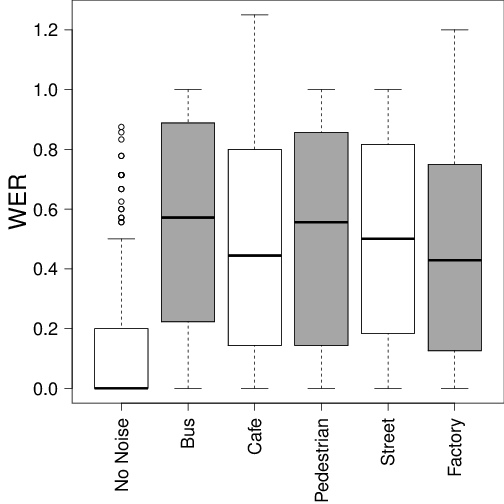
\includegraphics[width=\maxwidth]{figure/boxplot_noise-1} 

\caption{Boxplot displaying the average word error rate (WER) averaged over each participant for every noise type. WER is the variable on the y-axis, and noise type is on the x-axis.}
\label{fig:anova1_noise_boxplot}
\end{wrapfigure}
%
Figure \ref{fig:anova1_noiseXspkr_boxplot} and the interaction of noise type \textbf{x} mic location in Figure \ref{fig:anova1_noiseXmic_boxplot}.The conditions in which there is no noise present differs noticeably from those with noise; this can visually be seen even in the condition in which the speech was recorded at the ear. This is likely the root of the sphericity violations.

%\begin{wrapfigure}{L}{1\textwidth}
\begin{figure}[h!]

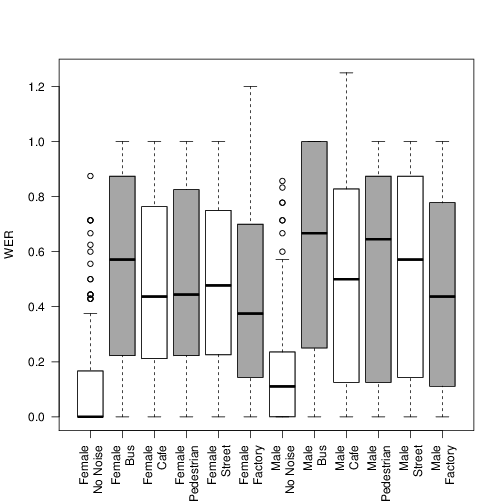
\includegraphics[width=\maxwidth]{figure/boxplot_noiseXspkr-1} 

\caption{Boxplot displaying the average word error rate (WER) averaged over each participant for the interaction of every noise type by the speaker gender. WER is the variable on the y-axis, and noise type by speaker gender is on the x-axis.}
\label{fig:anova1_noiseXspkr_boxplot}
\end{figure}

\begin{figure}[h!]%{L}{\textwidth}

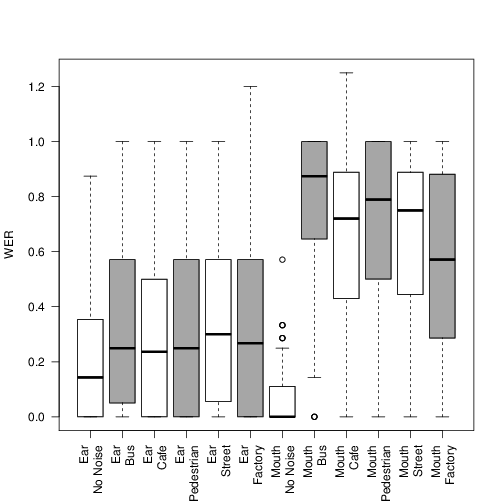
\includegraphics[width=\maxwidth]{figure/boxplot_noiseXmic-1} 

\caption{Boxplot displaying the average word error rate (WER) averaged over each participant for the interaction of every noise type by the mic location. WER is the variable on the y-axis, and noise type by mic location is on the x-axis.}
\label{fig:anova1_noiseXmic_boxplot}
\end{figure}


Since there is a statistical difference in the main effect of noise, and since the ``no noise'' condition is very apparently different from the other noise conditions, another ANOVA was calculated with the ``no noise'' level of noise type removed.  This was to test for statistical difference only in noise conditions containing actual noise (and any resulting interaction). This modified ANOVA is a two by two by five design, with the noise type factor only having 5 levels (with the ``no noise'' condition removed from the noise type factor).

The results are similar, with no significant three-way interaction, and - as before - two significant two-way interactions of speaker gender \textbf{x} mic location and noise-type \textbf{x} mic location (cf. Tables \ref{tab:anova2_by_subj} and \ref{tab:anova2_by_item}, respectively).  There are main effects of noise type and mic location.  The main effect of speaker gender differs from the first ANOVA in that it is only significant in the by-subjects ANOVA, but is not significant in the by-items ANOVAs.

% latex table generated in R 3.4.1 by xtable 1.8-2 package
% Sun Jul  9 18:16:32 2017
\begin{table}[ht]
\centering
\begin{tabular}{lrrrrl}
  \hline
Effect & DFn & DFd & F & p & p$<$.05 \\ 
  \hline
speaker\_gender & 1.00 & 23.00 & 5.26 & 0.03 & * \\ 
  noise\_type & 4.00 & 92.00 & 5.95 & 0.00 & * \\ 
  mic\_location & 1.00 & 23.00 & 215.08 & 0.00 & * \\ 
  speaker\_gender:noise\_type & 4.00 & 92.00 & 0.60 & 0.66 &  \\ 
  speaker\_gender:mic\_location & 1.00 & 23.00 & 16.68 & 0.00 & * \\ 
  noise\_type:mic\_location & 4.00 & 92.00 & 6.00 & 0.00 & * \\ 
  speaker\_gender:noise\_type:mic\_location & 4.00 & 92.00 & 1.14 & 0.34 &  \\ 
   \hline
\end{tabular}
\caption{ANOVA for by-subjects analysis of the three-factor, within-subjects experiment. The ``no noise'' condition was removed from the noise type factor, resulting in a 2x2x5 design.} 
\label{tab:anova2_by_subj}
\end{table}
% latex table generated in R 3.4.1 by xtable 1.8-2 package
% Sun Jul  9 18:16:32 2017
\begin{table}[ht]
\centering
\begin{tabular}{lrrrrl}
  \hline
Effect & DFn & DFd & F & p & p$<$.05 \\ 
  \hline
speaker\_gender & 1.00 & 71.00 & 3.46 & 0.07 &  \\ 
  noise\_type & 4.00 & 284.00 & 6.92 & 0.00 & * \\ 
  mic\_location & 1.00 & 71.00 & 515.73 & 0.00 & * \\ 
  speaker\_gender:noise\_type & 4.00 & 284.00 & 0.55 & 0.70 &  \\ 
  speaker\_gender:mic\_location & 1.00 & 71.00 & 20.62 & 0.00 & * \\ 
  noise\_type:mic\_location & 4.00 & 284.00 & 7.14 & 0.00 & * \\ 
  speaker\_gender:noise\_type:mic\_location & 4.00 & 284.00 & 1.35 & 0.25 &  \\ 
   \hline
\end{tabular}
\caption{ANOVA for by-items analysis of the three-factor, within-subjects experiment. The ``no noise'' condition was removed from the noise type factor, resulting in a 2x2x5 design.} 
\label{tab:anova2_by_item}
\end{table}


Again, Mauchley's Test for Sphericity was conducted, resulting only in a significant sphericity violation in the by-subjects ANOVA for noise (cf. Tables \ref{tab:anova2_subj_sph_test} and \ref{tab:anova2_item_sph_test}).  This was corrected with a Greenhouse-Geisser test, which resulted, again, in no changes to the determinations of statistical significance indicated in the ANOVAs in Tables \ref{tab:anova2_by_subj} and \ref{tab:anova2_by_item}.
% latex table generated in R 3.4.1 by xtable 1.8-2 package
% Sun Jul  9 18:16:32 2017
\begin{table}[ht]
\centering
\begin{tabular}{lrrl}
  \hline
Effect & W & p & p$<$.05 \\ 
  \hline
noise\_type & 0.26 & 0.00 & * \\ 
  speaker\_gender:noise\_type & 0.76 & 0.74 &  \\ 
  noise\_type:mic\_location & 0.58 & 0.23 &  \\ 
  speaker\_gender:noise\_type:mic\_location & 0.82 & 0.89 &  \\ 
   \hline
\end{tabular}
\caption{Sphericity test for the by-subjects ANOVA with the ``no noise'' condition removed.} 
\label{tab:anova2_subj_sph_test}
\end{table}
% latex table generated in R 3.4.1 by xtable 1.8-2 package
% Sun Jul  9 18:16:32 2017
\begin{table}[ht]
\centering
\begin{tabular}{lrrl}
  \hline
Effect & W & p & p$<$.05 \\ 
  \hline
noise\_type & 0.87 & 0.36 &  \\ 
  speaker\_gender:noise\_type & 0.88 & 0.43 &  \\ 
  noise\_type:mic\_location & 0.93 & 0.86 &  \\ 
  speaker\_gender:noise\_type:mic\_location & 0.98 & 1.00 &  \\ 
   \hline
\end{tabular}
\caption{Sphericity test for the by-items ANOVA with the ``no noise'' condition removed.} 
\label{tab:anova2_item_sph_test}
\end{table}



%(cf. Tables \ref{tab:anova2_subj_sph_corr} and \ref{tab:anova2_item_sph_corr}).

% # <<ANOVA2_sphericity_corr, echo=FALSE, results='asis'>>=
% # print(xtable(by_subj_ez_anova2$`Sphericity Corrections`, label="tab:anova2_subj_sph_corr", caption="Sphericity corrections for the by-subjects ANOVA with the ``no noise'' condition removed."), include.rownames=FALSE)
% # print(xtable(by_item_ez_anova2$`Sphericity Corrections`, label="tab:anova2_item_sph_corr", caption="Sphericity corrections for the by-items ANOVA with the ``no noise'' condition removed."), include.rownames=FALSE)
% # @




\section{Discussion}

% Points to hit here:
% X- Ear speech is more easily recognized than noisy speech from the mouth (print bar graph of mic loc simple effects)
% X- There is still a main effect of noise even when 'no noise' is removed, print bar graph w/ no 'no noise' and discuss simple effects
% X- Touch on 'near-significance' of speaker gender, how it isn't as near significant as it appears - likely an SNR effect (print graph).
% - Discuss noiseXmic interation data, re-print graph
% X-- Mention differences in mouth noise performance which come out in this interaction, medians ranging from approximately 60% (factory) to near 90% (bus); reference noise spectograms, give possible explanation
% X-- Non-noisy mouth speech is still the most easily recognized - median of zero - but non-noisy ear-speech does well for itself with a median nearing 15% WER.
% X-- There still appears to be a noticeable difference between ear-no noise and ear-noisy speech (some noise must get through), but no noticeable difference between noises within ear-speech category; nevertheless, median noisy ear-speech recognition appears to hover near 30% WER.
% X-- Comment on how this is evidence for ''predictable'' noise that is (more or less) non-varying between noise types.
% X- Look at longitudinal effects
% -- Surveys - add in later
% X- Move on to limitations
% -- Mention not all sound files had normalized amplitude - some were quite louder than others, which may be an explanation for some of the observed variability.
% -- Mention the computer screen distraction.


The primary hypotheses from Chapter 2\ref{chapter2} included (a) that the signal recorded from the ear, pre-emphasized, filtered, and pre-emphasized again, would be intelligible by human listeners, and (b) that it would be more intelligible than speech with a noisy background.  The results in Section \ref{ch4:results} above show a statistical difference between the WERs of the sentence transcriptions of the speech recorded from the ear canal and the speech recorded in front of the mouth.  This can be seen more clearly in the graph of the simple effects of microphone location, in Figure \ref{fig:mic_loc_simple}.  The speech recorded at the ear has a significantly lower transcription word error rate than the speech recorded at the mouth, collapsing over all noise conditions (this holds with or without clean speech). These primary hypotheses seem to have been validated.

A statistical interaction of speaker gender \textbf{x} mic location is found.  
Looking at a boxplot of this interaction in Figure \ref{fig:spkr-genXmic-loc}, it is apparent that the two genders have different effects on microphone location.  Based on this plot, it would appear that the female's ear-recorded speech offers less intelligibility benefit over the speech recorded at the mouth, while the male voice has more of a benefit.  This interaction seems to exist primarily because listeners are able to more accurately recognize the speech in noise when spoken by the female, rather than the male.
%
\begin{wrapfigure}{R}{0.5\textwidth}

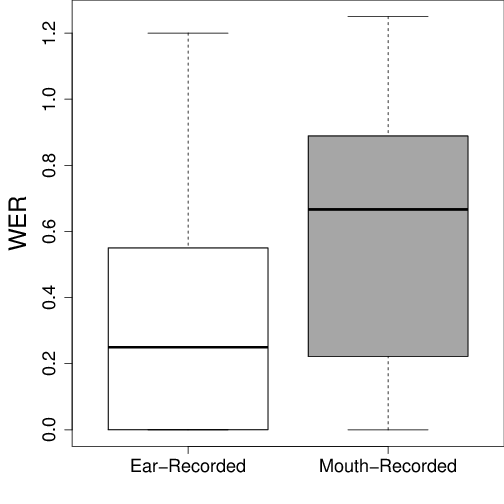
\includegraphics[width=\maxwidth]{figure/Mic-location_simple-1} 

\caption{Simple effects of Microphone Location.}
\label{fig:mic_loc_simple}
\end{wrapfigure}
%
However, while it is possible that gender itself is causing this effect, it should also noted that - in the instance of these two particular speakers - gender is confounded with level SNR.  The average female speaker's SNR in the speech recorded at mouth in noisy conditions was higher than the male speaker's SNR\footnote{\textbf{The only noise condition was 80 dB; the female speaker averaged less than +1 dB SNR and the male speaker averaged over +8 dB SNR, using the SNR calculator described in Section \textit{[Chapter 2: Ear Recorded Speech: Discussion]}\ref{chap2:discussion} and found in Appendix E\ref{appendixE}}}.


This likely contributed to the observed statistical difference.  If the SNR is high (as it was for the female's speech), the human auditory system can utilize the methods it has to ``release the masking'' in an effective manner.  Listeners therefore perform better on speech with richer frequency information (even if there is a bit of noise), than more distorted, ``muffled'' speech.  When the reverse is true and the speech in noise has a lower SNR (as it was in the male's speech), it cannot as easily be ``released from the masking'' by the auditory system.  Thus, speech that is slightly distorted - but has clearer harmonic and formant information - can be more easily understood.  The likelihood of the statistical difference seen being caused by SNR level also makes sense, as the major difference observed in Figure \ref{fig:spkr-genXmic-loc} occurs between the two genders' speech that is recorded at the mouth (in noisy conditions).  Unfortunately, this is only speculation, as with the given data, gender is confounded with SNR.

There is also a main effect of noise.  It is obvious that the speech recorded with no background noise (particularly at the mouth) would be easier to transcribe and recognize than the speech recorded with background noise.  However, when the level of `no noise' within the noise-type factor is removed, the statistical difference within this condition remains.

A closer look at the main effect of noise-type, excluding the level of `no noise', can be seen in Figure \ref{fig:noise-type_non-no-noise_main}.

The difference here is not nearly as stark as that seen within the microphone location distinction in Figure \ref{fig:mic_loc_simple}.  Even still, there is a observable difference, particularly between the bus background noise (with the highest relative WER) and the factory background noise (with the lowest relative WER).

Referring back to Figure \ref{fig:bkgrnd-noises}, containing the spectograms of the background noises in Section \ref{bkgrnd:speech_in_noise}, it appears that the bus noise (cf. Figure \ref{fig:fac-bkgrnd}) contains bands in the frequency spectrum that contain higher amplitude.
This may adversely affect a person's ability to parse the harmonics and/or formants from the desired speech. 

Again referring to Figure \ref{fig:bkgrnd-noises}, it is unclear, however, why the cafe background noise, among the other noises, has a relatively lower WER, since it also contains many more prominent bands of frequency from speaker babble. 
Similarly, it is difficult to observe much difference between the factory background noise and the pedestrian background noise, despite the pedestrian noise having a higher upper bound.

To see if any more apparent differences can be found, Figure \ref{fig:noiseXmic2} shows the noise type factor split between the two levels of mic location, displaying what was originally seen above in Figure \ref{fig:anova1_noiseXmic_boxplot}.  
%
\begin{wrapfigure}{l}{0.5\textwidth}

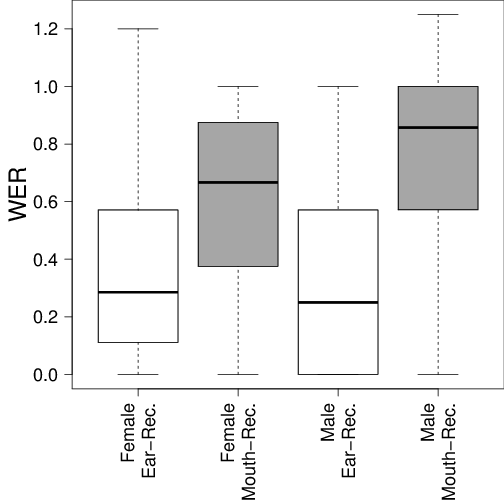
\includegraphics[width=\maxwidth]{figure/spkr-gender_mic-location_interaction-1} 

\caption{Interaction between speaker gender and microphone location.}
\label{fig:spkr-genXmic-loc}
\end{wrapfigure}
%
When only looking at the noise as it occurs in the mouth-recorded condition, the differences between the levels of noise become much more stark.  In particular, the difference between the bus noise (high WER) and factory noise (relatively lower WER) greatly expands. 

This distinction reaches as low as a median of approximately 60\% WER for the factory background noise conditions, and a median of nearly 90\% WER for the bus background noise.  The variance within noise conditions also differs, with the bus noise containing less variance (upper quartile 100\% WER, lower quartile ~68\% WER) than the factory noise condition (upper quartile ~90\% WER, lower quartile ~30\% WER).  The remaining noise conditions are more similar to one another, and fall in between the two, with median WERs hovering near 80\%.  The bus noise, as seen in Figure \ref{fig:bckgrnd-noises}, seems to contain very prominent frequency bands within the frequency range that is important for speech; it is possible that this plays a role in its noticeably higher WER.

The differences between the transcription WERs of the cafe, pedestrian, and street noises have expanded slightly, but still hover fairly close together in between the bus and factory performances. No explanation is proposed for the reason for these apparent divergences.

Out of all condition combinations in Figure \ref{fig:noiseXmic2}, the WER-front-runner is quite clearly the speech recorded at the mouth with no background noise.  There was never any doubt that this would be the case, as speech with relatively little background noise is the sort of speech from which learners acquire their language model, and whereby most communication occurs.  The median WER is, unsurprisingly, 0\%, though there is some variance from perfect perception; some errors do occasionally occur. 
%
\begin{wrapfigure}{l}{0.5\textwidth}

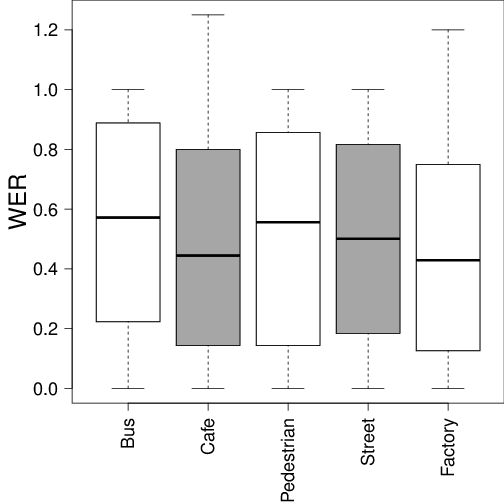
\includegraphics[width=\maxwidth]{figure/Noise-type_simple-1} 

\caption{Simple effects of Noise Type, excluding the level of `no noise'.}
\label{fig:noise-type_non-no-noise_main}
\end{wrapfigure}
%
The ear-recorded speech in a clean environment manages to also achieve a respectable transcription WER median of approximately 15\%, with a lower quartile boundary at 0\% WER and an upper quartile boundary of 35\% WER.

Despite being more similar than their mouth recorded counterparts, there is still a noticeable difference between the ear recorded speech with no noise, and ear recorded speech in noisy conditions.  Most noise conditions recorded from the ear achieve a lower quartile boundary near 0\%, but the upper quartile boundary for most nears 60\% WER.  The median WER for noise conditions generally falls at or slightly below 30\%. 

Even though there is a higher WER than the ear-recorded no-noise condition, the ear-recorded speech in noise is quite consistent across noise categories.  This is very different from the mouth-recorded speech in noise, which vary considerably between noise conditions.  This indicates that while a noise presence hampers transcription ability and increases WER in ear-recorded conditions, the varying qualities of the different background noises were dampened to the point of having a starkly lesser effect than that which occurs in the mouth-recorded speech.

Since the ability to recognize ear-recorded speech, even in noise, is quite consistent, the conditions are right for the auditory system to `perceptually learn' the distorted ear-recorded speech, as discussed in Section \ref{chap2:background} and by \cite{mattys:12}, among others.  This, in theory, would increase the learners' recognition of the ear-recorded speech with additional exposure, further increasing the WER improvement seen with ear-recorded speech.


\begin{figure}[h!]

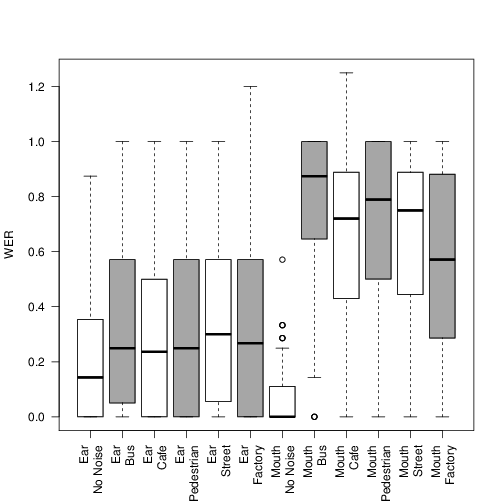
\includegraphics[width=\maxwidth]{figure/boxplot_noiseXmic2-1} 

\caption{Boxplot displaying the average word error rate (WER) averaged over each participant for the interaction of every noise type by the mic location. WER is the variable on the y-axis, and noise type by mic location is on the x-axis.}
\label{fig:noiseXmic2}
\end{figure}

To visualize whether the performance of participants generally improves over time, scatterplots graph participant's chronological performance with mouth-recorded and ear-recorded speech over the course of the experiment in Figures \ref{fig:linear_performance_m} and \ref{fig:linear_performance_e}. 
%
\begin{figure}[t]%{L}{0.5\textwidth}
\begin{subfigure}{0.47\textwidth}

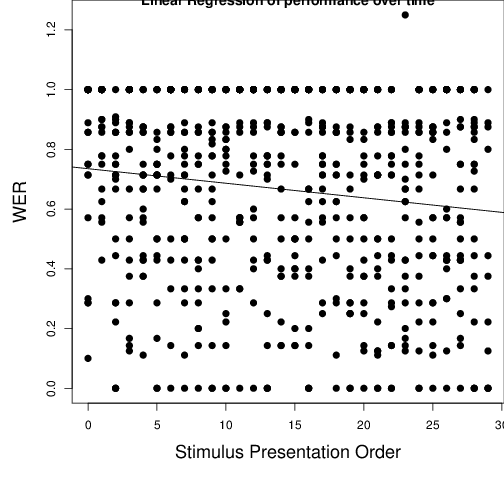
\includegraphics[width=\maxwidth]{figure/line_graph_chrono_m-1} 

\caption{Scatterplot of all participants' WER values for responses to speech recorded at the mouth \textbf{and} in noise.}
\label{fig:linear_performance_m}
\end{subfigure}
%\hfill
\begin{subfigure}{0.47\textwidth}%{L}{0.5\textwidth}

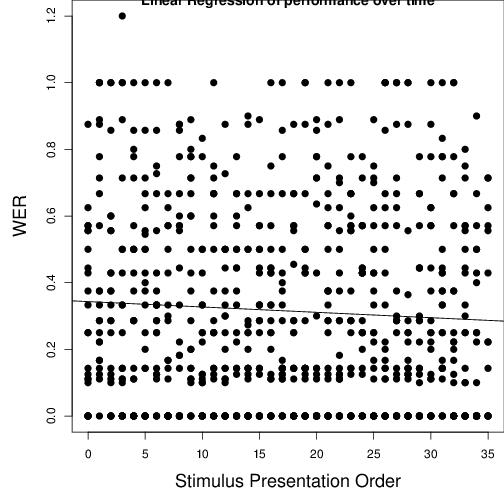
\includegraphics[width=\maxwidth]{figure/line_graph_chrono-1} 

\caption{Scatterplot of all participants' WER values for responses to speech recorded at the ear.}
\label{fig:linear_performance_e}
\end{subfigure}
\caption{The x-axis is the order of the responses; eg. ``1'' on the x-axis is the first response given by the participants.  The x-axis only corresponds to order of response, and does not indicate the specific noise type or gender of the speaker.  A line was fitted to the data using linear regression.}
\end{figure}
%
Linear regression models were fit onto the mouth-recorded data (slope=$-0.0048728$, $R^2$=$0.0175763$, $p<0.001$), and the ear-recorded data (slope=$-0.0016076$, $R^2$=$0.003146$, $p>0.05$). 

It is important to note the linear scales both axes, particularly the y-axis, as an explanation for why the slope values themselves are so small (ie. the y-axis range is from \textit{0.0} to \textit{1.2}).  The primary take away from both graphs and both fitted regression models in Figures \ref{fig:linear_performance_m} and \ref{fig:linear_performance_e} is that participants' recognition ability seems to improve statistically over the course of the experiment for mouth-recorded (noisy) speech, but not ear-recorded speech.  It could be possible that there are statistical gains by the noisy speech simply due to greater room for improvement, but it could also be due to the presence of high frequency speech information in the signal. The speech beneath the noise is ``normal'', containing full frequency information that the participant would be used to listening for, and if participants are able to use perceptual learning to take release the noise mask, this improvement over time is the expected effect.  However, as already seen, the overall performance on noisy, mouth recorded speech still falls well below that of ear-recorded speech, even at the end of the experiment.

%Of particular interest for the goals of this study, is the fact that - although very modest - there is improvement in recognition of ear-recorded speech that appears to correlate with an increase in exposure time to the ear-recorded speech.  That is, as more ear-recorded speech is heard, participants see modest gains in their ability to correctly recognize and transcribe it.  
One potential reason that there may not have been a statistical perceptual learning effect for ear-recorded speech over the course of the experiment is that the participant was not given feedback or the correct answer.  It has been shown (\cite{davis:05}) that such feedback can improve and speed up the perceptual learning process when listeners are able to correctly identify what was said.  This will be discussed further in Section \ref{ch4:follow-up-expts} below, and a follow up investigation will be conducted pertaining to this.


\subsection{Follow-up Investigations}
\label{ch4:follow-up-expts}

To expound on the previous study, two additional investigations were performed to give insights into possible future research directions.  The impetus for the first investigation was \cite{bird:97}, which demonstrated that fundamental frequency (F0) is a tool used by the auditory system to separate a desired source from masking noise.  This follow up proposes to recombine the very clear, lower frequencies from the ear-recorded speech with the ``noisy'' upper frequencies recorded at the mouth.  

The hypothesis is that the auditory system will use the clear fundamental frequency harmonic information in the lower frequencies to extract the upper harmonics out of the noise.  Accuracy is predicted to improve over that of the low-pass filtered, ``muffled'', ear speech (which many participants subjectively observed to be annoying and difficult to understand), as more high frequency information will be present and available for listeners' auditory systems.  This speech will sacrifice the advantage of being completely or nearly ``noise-free'', to sound more natural.  Additionally, since the ear-recorded speech consists of very clean harmonics, it is hypothesized that this speech, combined with the higher frequency mouth recorded speech in the noise-free condition, will perform equal to its mouth-recorded counterpart in the noise-free condition. This will be referred to as the ``F0'' investigation.

The second investigation was based on the concept of ``perceptual learning'' discussed earlier.  This presumes that the auditory system can learn to adapt to understand speech in a degraded signal better over time.  According to \cite{mattys:12}, significant learning can occur with even a small number of training trials.  \cite{davis:05} demonstrate that during training, successful recognition of a degraded signal will help one recognize a similar signal more than unsuccessful recognition of a degraded signal.  

Based on the implications of these findings, a short story was read and was recorded from inside the ear canal for the participants in this follow up study to listen to prior to completing the experiment itself.  This will serve as a brief ``training'' for participants in preparation for the actual task. Since the type of distortion from the ear-recorded signal is regular and predictable, it is hypothesized that perceptual learning will take place, and those who have listened to the training story will perform better on ear-recorded speech than those who had not (ie. those in the primary study). This will be referred to as the ``perceptual learning'' or ``training'' investigation.


\subsection{``F0'' Investigation Methods}
\label{F0-methods}

The stimuli used for this investigation consisted of the exact same sentences produced by the exact same speakers.  No modification was performed to the sentences recorded at the mouth.  For the sentences recorded at the ear, the same modifications as before (pre-emphasis, lowpass filtering\footnote{Lowpass filtered allowing 0-2500Hz, with a 500 Hz slope}, and a second pre-emphasis) were performed, but afterwards, the simultaneously recorded speech from the mouth was filtered and combined with the ear-recorded speech.  The speech from the mouth was bandpass filtered between 3000Hz and 8000Hz, with a 500Hz slope.  
%
\begin{wrapfigure}{r}{0.5\textwidth}
\centering
  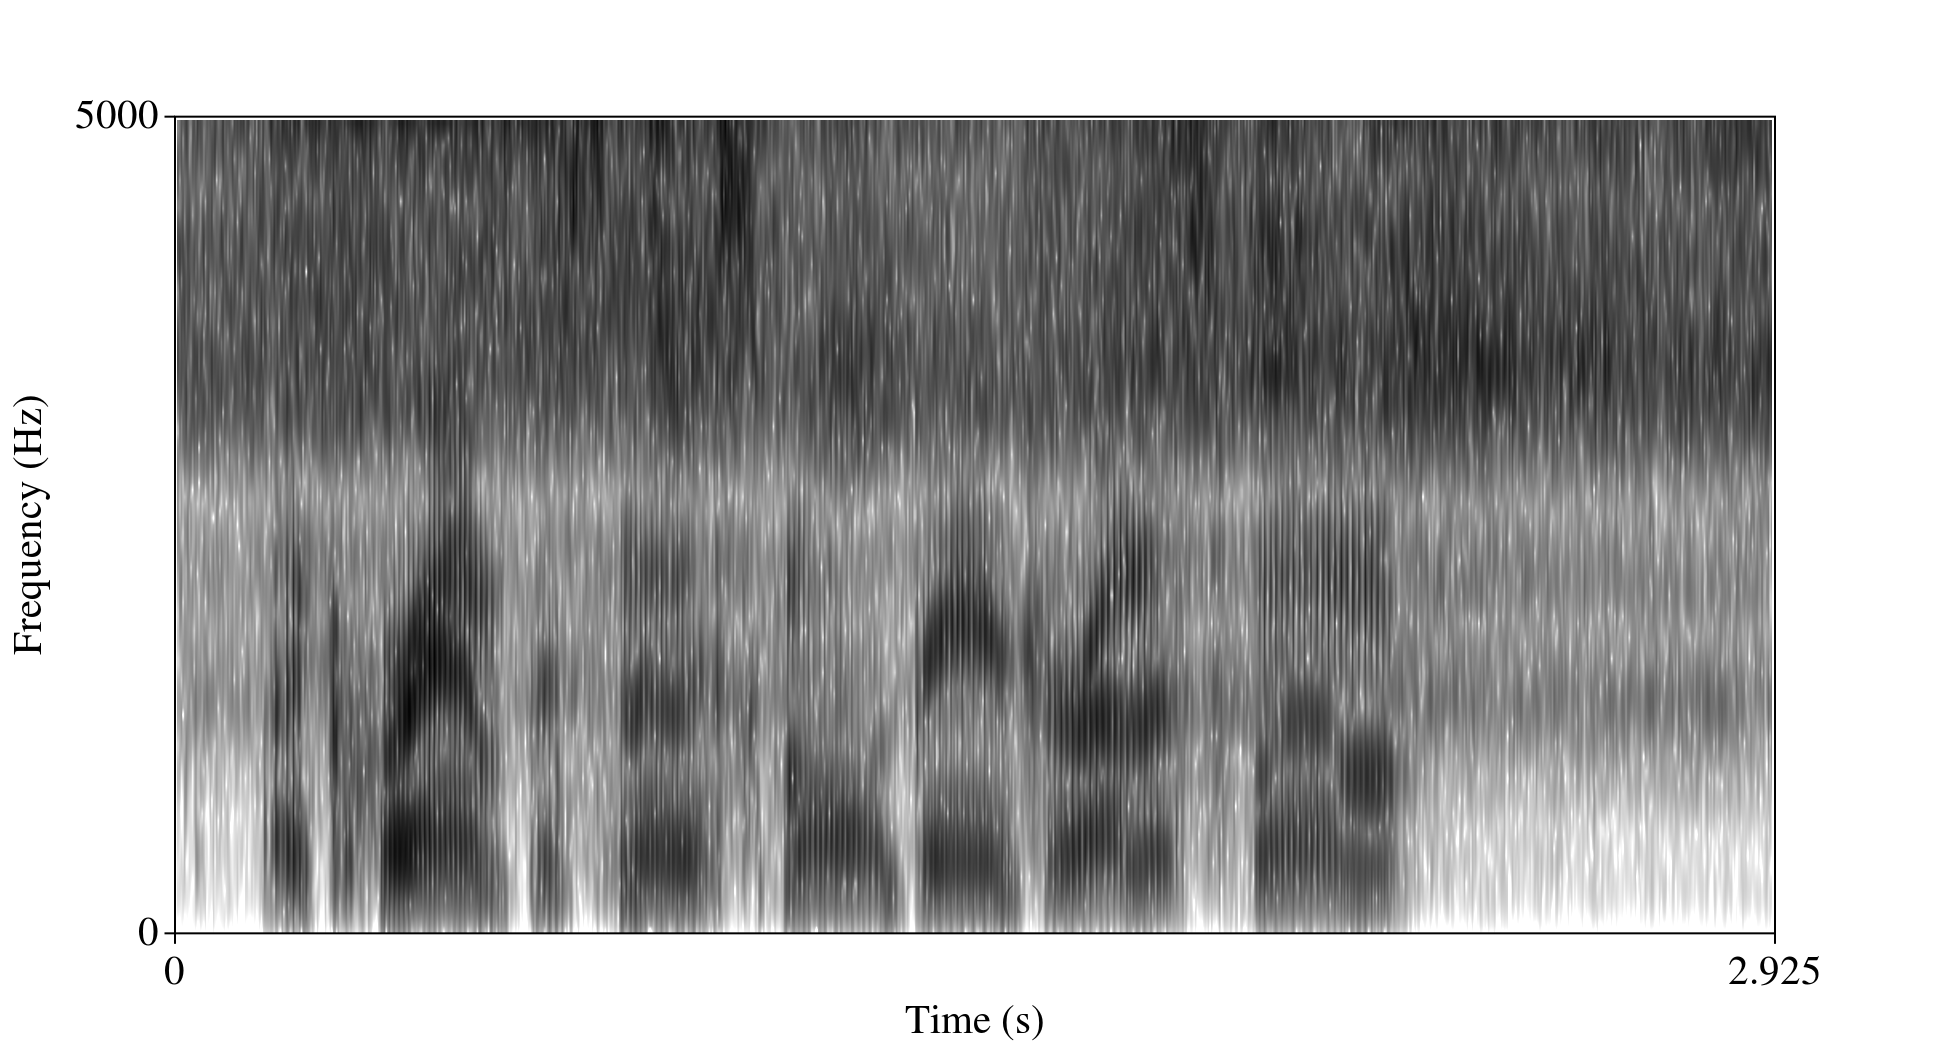
\includegraphics[width=0.45\textwidth]{figure/combined-signal.png}
  \caption{A spectrogram of the sentence ``A cramp is no small danger on a swim''.  The low-pass filtered ear-recorded signal was combined with the simultaneous [noisy] mouth signal, which was bandpass filtered at a higher frequency.}
  \label{fig:combined-signal}
\end{wrapfigure}
%
This allowed for an overlap of the frequencies from the mouth-recorded speech and the lowpass filtered ear-recorded speech.  The two signals were converted to a stereo signal, and then combined into a mono signal.  This resulted in relatively clean speech below approximately 2.7 kHz, and noisy speech above approximately 2.7 kHz, as seen in Figure \ref{fig:combined-signal}.

There were five native speakers of English with self-reported normal hearing who participated in this investigation.  The design and procedure of this task was exactly the same as the initial perception experiment, save the alteration in modifications performed on the ear-recorded stimuli, described above.


\subsection{``F0'' Results and Discussion}
\label{ch4:F0_discussion}

%\begin{wrapfigure}{L}{0.75\textwidth}

% \caption{Using the data from the five participants who performed the experiment using the speech in which the higher frequencies were added back in from the noisy mouth-recorded speech.  Boxplot displaying the average word error rate (WER) averaged over each participant for every noise type. WER is the variable on the y-axis, and noise type is on the x-axis.}
% \label{fig:F0_noise_boxplot}
% \end{wrapfigure}

% \begin{figure}%{L}{\textwidth}
% <<F0_boxplot_noiseXspkr, echo=FALSE, results='asis'>>=
% boxplot(wer~noise_type*speaker_gender,col=c("white","lightgray"),F0data, names=c("Female\nNo Noise","Female\nBus","Female\nCafe","Female\nPedestrian","Female\nStreet","Female\nFactory","Male\nNo Noise","Male\nBus","Male\nCafe","Male\nPedestrian","Male\nStreet","Male\nFactory"),ylab="WER",las=2)
% @
% \caption{Using the data from the five participants who performed the experiment using the speech in which the higher frequencies were added back in from the noisy mouth-recorded speech.  Boxplot displaying the average word error rate (WER) averaged over each participant for the interaction of every noise type by the speaker gender. WER is the variable on the y-axis, and noise type by speaker gender is on the x-axis.}
% \label{fig:F0_noiseXspkr_boxplot}
% \end{figure}

\begin{figure}[h!]%{L}{\textwidth}

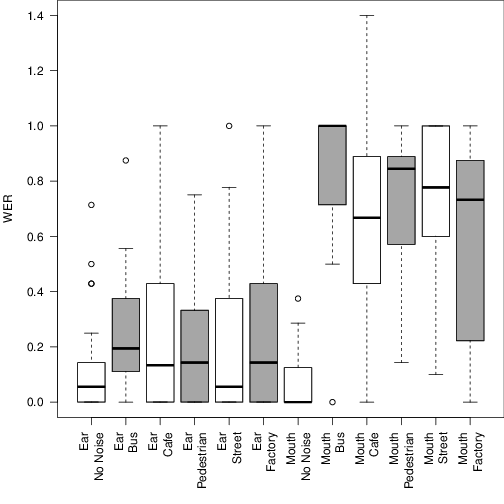
\includegraphics[width=\maxwidth]{figure/F0_boxplot_noiseXmic-1} 

\caption{Using the data from the five participants who performed the task using the speech in which the higher frequencies were added back in from the noisy mouth-recorded speech.  Boxplot displaying the average word error rate (WER) averaged over each participant for the interaction of every noise type by the mic location. WER is the variable on the y-axis, and noise type by mic location is on the x-axis.}
\label{fig:F0_noiseXmic_boxplot}
\end{figure}

Since there were only five participants in this follow-up investigation, no actual statistics were run to test for significance.  The results here are to be used in a basic comparison of possible directions these altered methods may be able to take future research.

The boxplot in Figure \ref{fig:F0_noiseXmic_boxplot} demonstrates the interaction of most interest, that of noise-type and microphone location, as identified by the ANOVAs performed on the primary experiment above.  No change was made to any of the presented mouth-recorded speech signals, so, as is observed, one would not expect there to be any change to listeners' ability to recognize these signals (outside of expected inter-speaker variation).

It is interesting to note that the primary difference between the clean ear-recorded speech and the ``noisy'' ear-recorded speech appears to be the extent of the variation in the upper quartile and whiskers.  Based on what is seen here, if this follow up study were to be extended carried out in a full study, one would expect there to be a dramatic difference between the noisy speech recorded at the mouth, and the speech recorded at the ear.
Further discussion concerning the comparison of these results with those of the primary study and the ``perceptual learning'' study can be found below in Section \ref{ch4:glob_discussion}.
% %
% \begin{wrapfigure}{L}{0.5\textwidth}
% <<F0spkr-gender_mic-location_interaction, echo=FALSE, results='asis'>>=
% boxplot(wer~speaker_gender*mic_location,col=c("white","lightgray"),F0data, names=c("Female\nEar-Recorded","Female\nMouth-Recorded","Male\nEar-Recorded","Male\nMouth-Recorded"),ylab="WER")
% @
% \caption{Interaction between speaker gender and microphone location.}
% \label{fig:F0_spkr-genXmic-loc}
% \end{wrapfigure}
% %


\subsection{``Perceptual Learning'' Methods}

For this investigation, a new speaker was recorded from the ear canal (with the same set-up as all previous recordings) reciting the short story ``Peter Rabbit'', by Beatrix Potter.  The recorded story, as was presented to the participants, had a total length of approximately 5 minutes and 13 seconds.  The recorded story underwent the same transformations as the ear-recorded stimuli in the primary study (ie. pre-emphasis, lowpass filtering\footnote{Lowpass filter of 0-2500Hz with a 500Hz slope.}, and pre-emphasis again).

There were four native speakers of English with self-reported normal hearing who participated in this follow up investigation.  They were first presented with a transcript of the story, and asked to listen to the audio and read along.  This offers ample chance for ``successful'' recognition of the degraded ear-recorded signal (cf. \cite{davis:05}).  After the reading session, the participants conducted the task as was done in the other tasks mentioned in Sections \ref{hsp-main-procedure} and \ref{F0-methods}, with the exact same stimuli as in the primary experiment.

\subsection{``Perceptual Learning'' Results and Discussion}

%\begin{wrapfigure}{L}{0.75\textwidth}

% \caption{Using the data from the four participants who performed the training task in which they listened and read along to a story prior to the experiment.  Boxplot displaying the average word error rate (WER) averaged over each participant for every noise type. WER is the variable on the y-axis, and noise type is on the x-axis.}
% \label{fig:perc_noise_boxplot}
% \end{wrapfigure}

% \begin{wrapfigure}{L}{\textwidth}
% <<perc_boxplot_noiseXspkr, echo=FALSE, results='asis'>>=
% boxplot(wer~noise_type*speaker_gender,col=c("white","lightgray"),perc_data, names=c("Female\nNo Noise","Female\nBus","Female\nCafe","Female\nPedestrian","Female\nStreet","Female\nFactory","Male\nNo Noise","Male\nBus","Male\nCafe","Male\nPedestrian","Male\nStreet","Male\nFactory"),ylab="WER",las=2)
% @
% \caption{Using the data from the four participants who performed the training task in which they listened and read along to a story prior to the experiment.  Boxplot displaying the average word error rate (WER) averaged over each participant for the interaction of every noise type by the speaker gender. WER is the variable on the y-axis, and noise type by speaker gender is on the x-axis.}
% \label{fig:perc_noiseXspkr_boxplot}
% \end{wrapfigure}

\begin{figure}[h!]

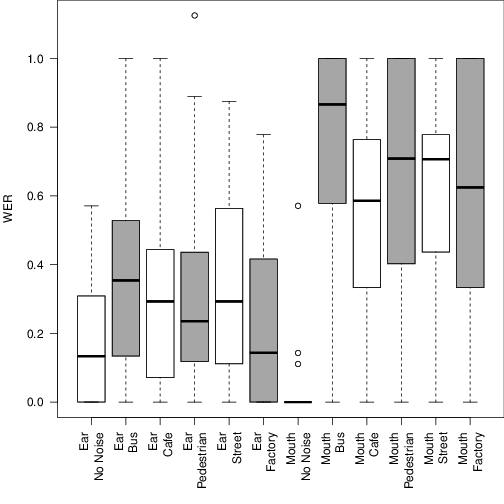
\includegraphics[width=\maxwidth]{figure/perc_boxplot_noiseXmic-1} 

\caption{Using the data from the four participants who performed the training task in which they listened and read along to a story prior to the experiment. Boxplot displaying the average word error rate (WER) averaged over each participant for the interaction of every noise type by the mic location. WER is the variable on the y-axis, and noise type by mic location is on the x-axis.}
\label{fig:perc_noiseXmic_boxplot}
\end{figure}

As stated in the discussion of the ``F0'' investigation in Section \ref{ch4:F0_discussion}, there are too few participants to run actual statistics on the results of this follow up investigation, and so implications here should be taken lightly and used to prepare further future research in this area. The only difference between this investigation and the primary study are that the participants in this task heard a 5 minute, 13 second ``training'' story beforehand, recorded from the story narrator's ear.

The boxplot in Figure \ref{fig:perc_noiseXmic_boxplot} displays the interaction of noise type and microphone location, which was a statistical interaction in the primary experiment.  It can be seen that the relationship between ear- and noisy mouth-recorded speech appear to remain the same; as expected the ear-recorded speech continues to be more easily recognized than speech recorded at the mouth in noise.  Further discussion continues below.



\subsection{Discussion of All Investigations}
\label{ch4:glob_discussion}

Looking into the differences between the primary study and the two follow-up studies, Figure \ref{fig:ALLXperc_noiseXmic_mouth_boxplot} shows the difference between the mouth-recorded speech in each of these three studies.  Given that no change was actually made to the audio of the mouth-recorded speech between these different experiments, there is expected to be no significant visual difference between the three different sets of boxplots, which is largely what is seen.  The participants in the ``perceptual learning'' task did perform remarkably well when recognizing clean speech from the mouth compared to the other studies, but this would be expected to be washed out with a proper number of participants.

\begin{figure}[h!]

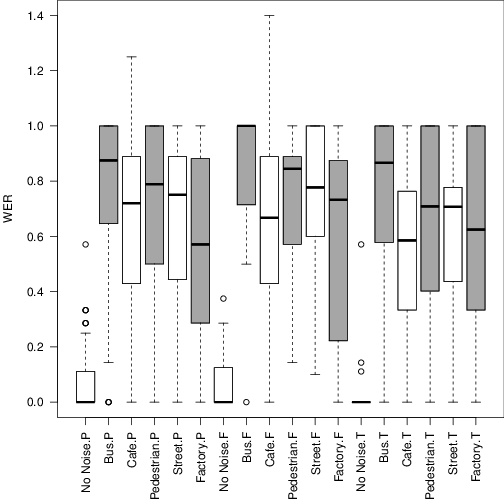
\includegraphics[width=\maxwidth]{figure/boxplot_noiseXmicXall_mouth-1} 

\caption{Boxplot displaying the average word error rate (WER) averaged over each participant for the interaction of every noise type by the mic location, for all three studies. Only data from mouth-recorded speech is shown. WER is the variable on the y-axis, and noise type by mic location is on the x-axis. P = `Primary' study; F = `F0' study; T = `Training' study}
\label{fig:ALLXperc_noiseXmic_mouth_boxplot}
\end{figure}

The minor differences that can be visually observed in the noisy speech conditions recorded at the mouth are expected to be washed out as well.  It is possible that the study involving the training task, exposing listeners to degraded speech, would help `train' their auditory system to be more perceptive overall, but this is not expected to result in significant benefit.

Moving on to the speech recorded at the ear in each study, these comparisons can be seen in Figure \ref{fig:ALLXperc_noiseXmic_ear_boxplot}.  By reintroducing noise into the signal, the results of the `F0' study could have potentially gone in either direction.  However, the recognition WER from the `Training' study would not be expected to be higher than that of the primary study, because the stimuli in both studies are exactly the same.  

This is precisely what is seen; while there are some variances (and increased variance between the individual noise types), the data from the `Training' study seems to result in essentially the same results the primary study.  A full-fledged study with more participants is certainly needed to be able to make any inferences about the benefits of this particular training procedure, but the results shown here do not indicate much improvement.  There are a number of potential factors that may have, or could in the future affect the ability of listeners to fully benefit from the training offered.  

While unlikely a major component, a single, different (male) voice was used for the training story in this follow-up study.  It is possible that the use of only one voice did not provide listeners with an adequate variety of vocal variations to make proper inferences about the distortion.  It is also important to consider the use of at least one male and at least one female voice during training, to avoid a potential gender effect.

Additionally, while for this task full attention was assumed, it is uncertain how much actual attention participants were devoting to listening to the training story.  Rather than a ``read-along'' training task, a more interactive task may capture more attention than passive listening and reading.  The interactive task could be structured as a forced decision task, providing multiple choice answers to an ear recorded sentence they hear.  Alternatively, it could be structured (as in the experiment itself) to force listeners to ``fill in the blank'' with what they thought was spoken, then provide listeners with the feedback in the form of the answer.  

In either of these tasks, the listener should be given the ability to replay the same sound multiple times.  The length of time in a ``read-along'' training task, or the number of training sentences in an interactive training task, would also likely have an effect on sentence recognition during the experiment.  This should be determined more carefully than was done in the above experiment.

\begin{figure}[h!]

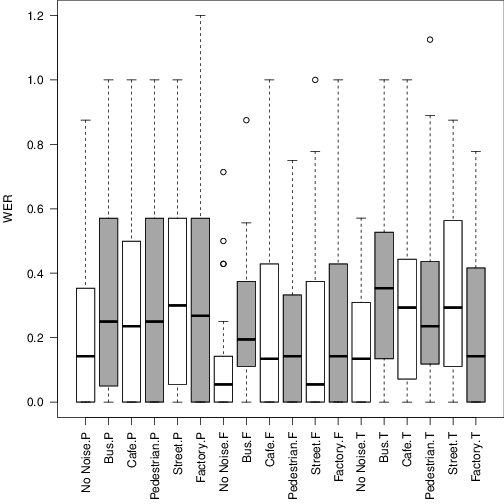
\includegraphics[width=\maxwidth]{figure/boxplot_noiseXmicXall_ear-1} 

\caption{Boxplot displaying the average word error rate (WER) averaged over each participant for the interaction of every noise type by the mic location, for all three studies. Only data from ear-recorded speech is shown.  WER is the variable on the y-axis, and noise type by mic location is on the x-axis. P = `Primary' study; F = `F0' study; T = `Training' study}
\label{fig:ALLXperc_noiseXmic_ear_boxplot}
\end{figure}

The `F0' experiment, also displayed in Figure \ref{fig:ALLXperc_noiseXmic_ear_boxplot}, appears to genuinely have promise.  It would be expected that the `non-noise' condition would perform much better under this transformation, since \textit{clean} upper frequency information is being added back into the signal (ie. there is no additional noise being added, only information that was previously lost).  

In the conditions in which there is noise, it was uncertain whether there would be benefit - and if so, to what degree - of re-incorporating noisy upper frequencies.  Yet there appears to be a noticeable performance increase.  For every individual noise type, the median WER in the `F0' study is lower than that in the primary study. 

There is often important (though, perhaps, not critical) speech information above the ~2700 Hz lowpass cutoff imposed on the stand-alone ear-recorded speech.  This would be expected, as a standard bandpassed signal for a telephone reaches up to 3500 Hz, and there are still those who have difficulty with its intelligibility.  The noisy upper frequencies which were added back into the ear-recorded signal contain this important information.  These preliminary results indicate that the human auditory system seems to be adept enough to parse this speech information from the higher frequencies out of the surrounding background noise using the ``clearer'' speech information in the lower frequencies.  And, importantly, that this benefits recognition.

Further investigation, of course, is still needed, as these preliminary WERs from the F0 study are from only five listeners.  Additionally, this method is still (albeit to a lesser degree) at the mercy of the ambient noise, and one would expect that as the SNR decreases (ie. as the noise level increases), this method will become less effective, and the auditory system poorer at extracting the high frequency speech information from the noise.  The range of SNRs at which this method becomes ineffective, as well statistically demonstrating its effectiveness in general, will need to be carried out by future research.

\subsection{Limitations}

There are several limitations that were noted during the experiment.  The first was brought up by a participant during discussion while filling out a questionnaire, and, while minor, has interesting ties to the literature.  This participant (including several others), mentioned the fact that they found the task particularly difficult due to the computer monitor in front of them.  The participant reported that it was difficult to focus on recognition of the stimulus due to the glow and competing visual stimulus of the computer monitor.

This is in line with what was found in \cite{francis:09} and \cite{francis:10} concerning working memory and perception; in this instance staring at the computer monitor and resulting visual stimulation proved to be a distraction and overloaded the working memory of the participant, which was already overloaded by trying to interpret the noisy and degraded speech.  Remarkably several participants commented that the computer monitor proved to be a distraction.  This diversion of working memory may have had a detrimental effect on recognition (cf. \cite{caplan:99}).

Another limitation, realized partway through the experiment, was that not all of the sound files had a normalized amplitude.  There were some which the amplitude of the sound was below what it should have been, and some in which this amplitude was greater than it should have been.  This occurred seemingly randomly throughout all conditions, and likely resulted in more variance towards the higher WERs and poorer performance on these sentences with ``abnormal'' amplitudes.

Notably, the number of participants per counter-balanced group is rather low.  There are 24 total participants, but only one in each counter-balanced group.  This means that only one person heard each individual sentence in a given condition combination\footnote{For example, only one person heard ``A cramp is no small danger on a swim'' spoken by the male speaker, recorded at the mouth with bus background noise; this is true of all sentence/condition combinations.}.  If more participants were able to be run in each counter-balanced group, this would present a more accurate representation of performance on a given item, rather than having only one WER for each sentence-condition combination.

Additionally, as stated earlier in Sections \textit{\textbf{[First Chapter, Limitations]}}\ref{ch2:limitations} and \ref{chap4:methods:stimuli}, the method of recording these stimuli to achieve a higher SNR ratio\footnote{Recall, the microphone in front of the mouth was pointed towards the loudspeaker} may have artificially increased some of the differences seen between the noisy speech recorded at the mouth and the same speech recorded at the ear.  Since there still appears to be some noise that reaches the microphone at the ear (there is a difference between the noisy conditions at the ear and the non-noise condition at the ear), this may have had a detrimental effect on listener's performance on these sentences.  Future research could avoid this by increasing the ambient noise using a capable loudspeaker with appropriate hearing protection for both participant and researcher, and in an environment where the surrounding environment can be insulated from this level of noise (cf. Section \textit{\textbf{[First Chapter, Limitations]}}\ref{ch2:limitations} for more details).


% \section{Survey Results}

% # <<survey_results_load, echo=FALSE, results='asis'>>=
% # exp2_data1 <- read.csv("/home/sam/Dissertation/exp2_data.csv")
% # exp2_data2 <- read.csv("/home/sam/Dissertation/exp2_inelligible_data.csv")
% # 
% # exp2_data <- rbind(exp2_data1,exp2_data2)
% # 
% # exp2_data$difficult[exp2_data$difficult == "y"] <- "yes"
% # exp2_data$difficult[exp2_data$difficult == "s"] <- "somewhat"
% # exp2_data$difficult[exp2_data$difficult == "n"] <- "no"
% # 
% # exp2_data$nois_muff[exp2_data$nois_muff == "n"] <- "noisy"
% # exp2_data$nois_muff[exp2_data$nois_muff == "b"] <- "both"
% # exp2_data$nois_muff[exp2_data$nois_muff == "m"] <- "muffled"
% # 
% # exp2_data$muff_annoy[exp2_data$muff_annoy == "y"] <- "yes"
% # exp2_data$muff_annoy[exp2_data$muff_annoy == "s"] <- "somewhat"
% # exp2_data$muff_annoy[exp2_data$muff_annoy == "n"] <- "no"
% # 
% # ggplot(exp2_data$nois_muff, aes(x=variable)) + geom_bar()
% # @

% The 24 participants in the primary study were asked 3 questions, (a) ``Overall did you find the task difficult?'', (b) ``Which did you find more difficult, the noisy speech or the `muffled' speech?'', and (c) ``Would you find it uncomfortable/annoying to listen to the muffled speech for an extended period?''.  Qualitative answers were given, which were then coded into different categories by a researcher.  Regarding question (a), 18 participants found the task to be difficult, while 8 found it to be \textit{somewhat} difficult.  No one responded that the task was easy.  
% 
% For question (b), the `muffled' speech refers to the ear-recorded speech, which the participants were unaware was recorded from the ear.  There were 14 responses which deemed the noisy speech more difficult to understand and 10 responses that deemed the muffled speech more difficult to understand.  Two respondants reported that both were equally difficult.  This is particularly interesting, because while subjectively responses were relatively split between the two recording locations (noisy speech from the mouth, and `muffled' speech from the ear), every single participant had a lower WER for the ear-recorded speech compared to their WER for the noisy, mouth-recorded speech.  This means that their subjective judgement of overall intelligibility did not match their sentence-for-sentence recognition performance.
% 
% Question (c), however, shows a one-sided agreement similar to question (a); 18 participants reported that they would find it annoying or uncomfortable to listen to the `muffled' ear-recorded speech for an extended period of time.  There were 5 respondants who reported it would only be \textit{somewhat} annoying/uncomfortable, and 3 respondants who said it would not be uncomfortable to listen to the `muffled' speech.  The 8 participants who answered ``somewhat'' or ``no'' for question (c) do not necessarily correspond with the 8 participants who answered ``somewhat'' in question (a).
% 
% This same survey was completed by the four participants in the ``perceptual-learning'' investigation.  Question (a) resulted in 3 ``yes'' answers and 1 ``somewhat'' answer.  Question (b) yielded 3 participants who believed the noisy speech was more difficult to understand, and 1 participant who thought the `muffled' speech was more difficult.  All four participants reported that they would find it annoying or uncomfortable to listen to the muffled speech for longer periods of time.  These answers are given despite the training task they performed, listening and reading a story in which the narration was recorded from the speaker's ear.  Similar to the preliminary results seen in Figure \ref{}, the training seems to have had no effect on listener's ability to understand, or comfort with, speech recorded from the ear.


\section{Conclusion}

In summary, speech recorded at the ear, via the process described in Chapter 2\ref{chapter2} does appear to be intelligible by human listeners, despite being severely low-pass filtered.  More-so, it is more intelligible than simultaneously recorded speech at the mouth in noise, although mouth-recorded speech without background noise is still obviously the easiest to understand.  A speaker gender interaction was found to be significant, but this is likely due to differences in the SNR for each speaker, rather than their gender.  

The additional follow-up study using training to help listeners become more accustomed to the ear-recorded speech did not demonstrate much performance over training.  However, the additional follow up study which recombined the high frequency information from the mouth-recorded speech with the low-pass filtered ear-recorded speech indicates that this transformation might yield greater human recognition of speech than the ear-recorded signals by themselves.

It is important to emphasize that the results from both the follow-up studies are not statistically significant, simply because they did not contain enough participants to run statistics.  Future research should expand on these preliminary results, conducting more thorough and statistical experimentation\footnote{\textbf{Stimuli, experimental code, and data from this experiment can be found at URL.COM}}.  There are certainly more stimuli modifications to explore that exploit the auditory system's innate ability to release it from the masking of ambient noise.

\bibliographystyle{apa}
\bibliography{DissRefs.bib}
\end{document}
